\documentclass[]{article}
\usepackage{lmodern}
\usepackage{amssymb,amsmath}
\usepackage{ifxetex,ifluatex}
\usepackage{fixltx2e} % provides \textsubscript
\ifnum 0\ifxetex 1\fi\ifluatex 1\fi=0 % if pdftex
  \usepackage[T1]{fontenc}
  \usepackage[utf8]{inputenc}
\else % if luatex or xelatex
  \ifxetex
    \usepackage{mathspec}
  \else
    \usepackage{fontspec}
  \fi
  \defaultfontfeatures{Ligatures=TeX,Scale=MatchLowercase}
\fi
% use upquote if available, for straight quotes in verbatim environments
\IfFileExists{upquote.sty}{\usepackage{upquote}}{}
% use microtype if available
\IfFileExists{microtype.sty}{%
\usepackage{microtype}
\UseMicrotypeSet[protrusion]{basicmath} % disable protrusion for tt fonts
}{}
\usepackage[margin=1in]{geometry}
\usepackage{hyperref}
\hypersetup{unicode=true,
            pdftitle={Can soil respiration measured at MAT represent annual soil respiration?},
            pdfauthor={Jinshi},
            pdfborder={0 0 0},
            breaklinks=true}
\urlstyle{same}  % don't use monospace font for urls
\usepackage{graphicx,grffile}
\makeatletter
\def\maxwidth{\ifdim\Gin@nat@width>\linewidth\linewidth\else\Gin@nat@width\fi}
\def\maxheight{\ifdim\Gin@nat@height>\textheight\textheight\else\Gin@nat@height\fi}
\makeatother
% Scale images if necessary, so that they will not overflow the page
% margins by default, and it is still possible to overwrite the defaults
% using explicit options in \includegraphics[width, height, ...]{}
\setkeys{Gin}{width=\maxwidth,height=\maxheight,keepaspectratio}
\usepackage[normalem]{ulem}
% avoid problems with \sout in headers with hyperref:
\pdfstringdefDisableCommands{\renewcommand{\sout}{}}
\IfFileExists{parskip.sty}{%
\usepackage{parskip}
}{% else
\setlength{\parindent}{0pt}
\setlength{\parskip}{6pt plus 2pt minus 1pt}
}
\setlength{\emergencystretch}{3em}  % prevent overfull lines
\providecommand{\tightlist}{%
  \setlength{\itemsep}{0pt}\setlength{\parskip}{0pt}}
\setcounter{secnumdepth}{0}
% Redefines (sub)paragraphs to behave more like sections
\ifx\paragraph\undefined\else
\let\oldparagraph\paragraph
\renewcommand{\paragraph}[1]{\oldparagraph{#1}\mbox{}}
\fi
\ifx\subparagraph\undefined\else
\let\oldsubparagraph\subparagraph
\renewcommand{\subparagraph}[1]{\oldsubparagraph{#1}\mbox{}}
\fi

%%% Use protect on footnotes to avoid problems with footnotes in titles
\let\rmarkdownfootnote\footnote%
\def\footnote{\protect\rmarkdownfootnote}

%%% Change title format to be more compact
\usepackage{titling}

% Create subtitle command for use in maketitle
\providecommand{\subtitle}[1]{
  \posttitle{
    \begin{center}\large#1\end{center}
    }
}

\setlength{\droptitle}{-2em}

  \title{Can soil respiration measured at MAT represent annual soil respiration?}
    \pretitle{\vspace{\droptitle}\centering\huge}
  \posttitle{\par}
    \author{Jinshi}
    \preauthor{\centering\large\emph}
  \postauthor{\par}
      \predate{\centering\large\emph}
  \postdate{\par}
    \date{March 26, 2019}

\usepackage{booktabs}
\usepackage{longtable}
\usepackage{array}
\usepackage{multirow}
\usepackage{wrapfig}
\usepackage{float}
\usepackage{colortbl}
\usepackage{pdflscape}
\usepackage{tabu}
\usepackage{threeparttable}
\usepackage{threeparttablex}
\usepackage[normalem]{ulem}
\usepackage{makecell}
\usepackage{xcolor}

\begin{document}
\maketitle

\hypertarget{the-spatial-distribution-of-global-rs-sites}{%
\section{1. The spatial distribution of global Rs
sites}\label{the-spatial-distribution-of-global-rs-sites}}

\begin{itemize}
\item
  In daily and monthly time scale, we used this approach a lot
  Rs\_mat\_Rs\_diurnal ()
  \includegraphics{6-Bahn_Analysis_Report_files/figure-latex/unnamed-chunk-1-1.pdf}
  \includegraphics{6-Bahn_Analysis_Report_files/figure-latex/unnamed-chunk-1-2.pdf}
\item
  We have much more measurements Rs in mid-latitude regions, where
  developed countries are mostly located
\item
  It is difficult to measure soil respiration all year around in cold
  regions, but critical because of high rates of climate change and
  large soil C stocks
\item
  Less-developed countries are constrained by lack of resources, and
  thus we do not have enough measurements from tropical regions
  \href{http://dx.doi.org/10.1016/j.jplph.2016.08.007}{(Xu and Shang
  2016)}
\end{itemize}

\begin{figure}
\centering
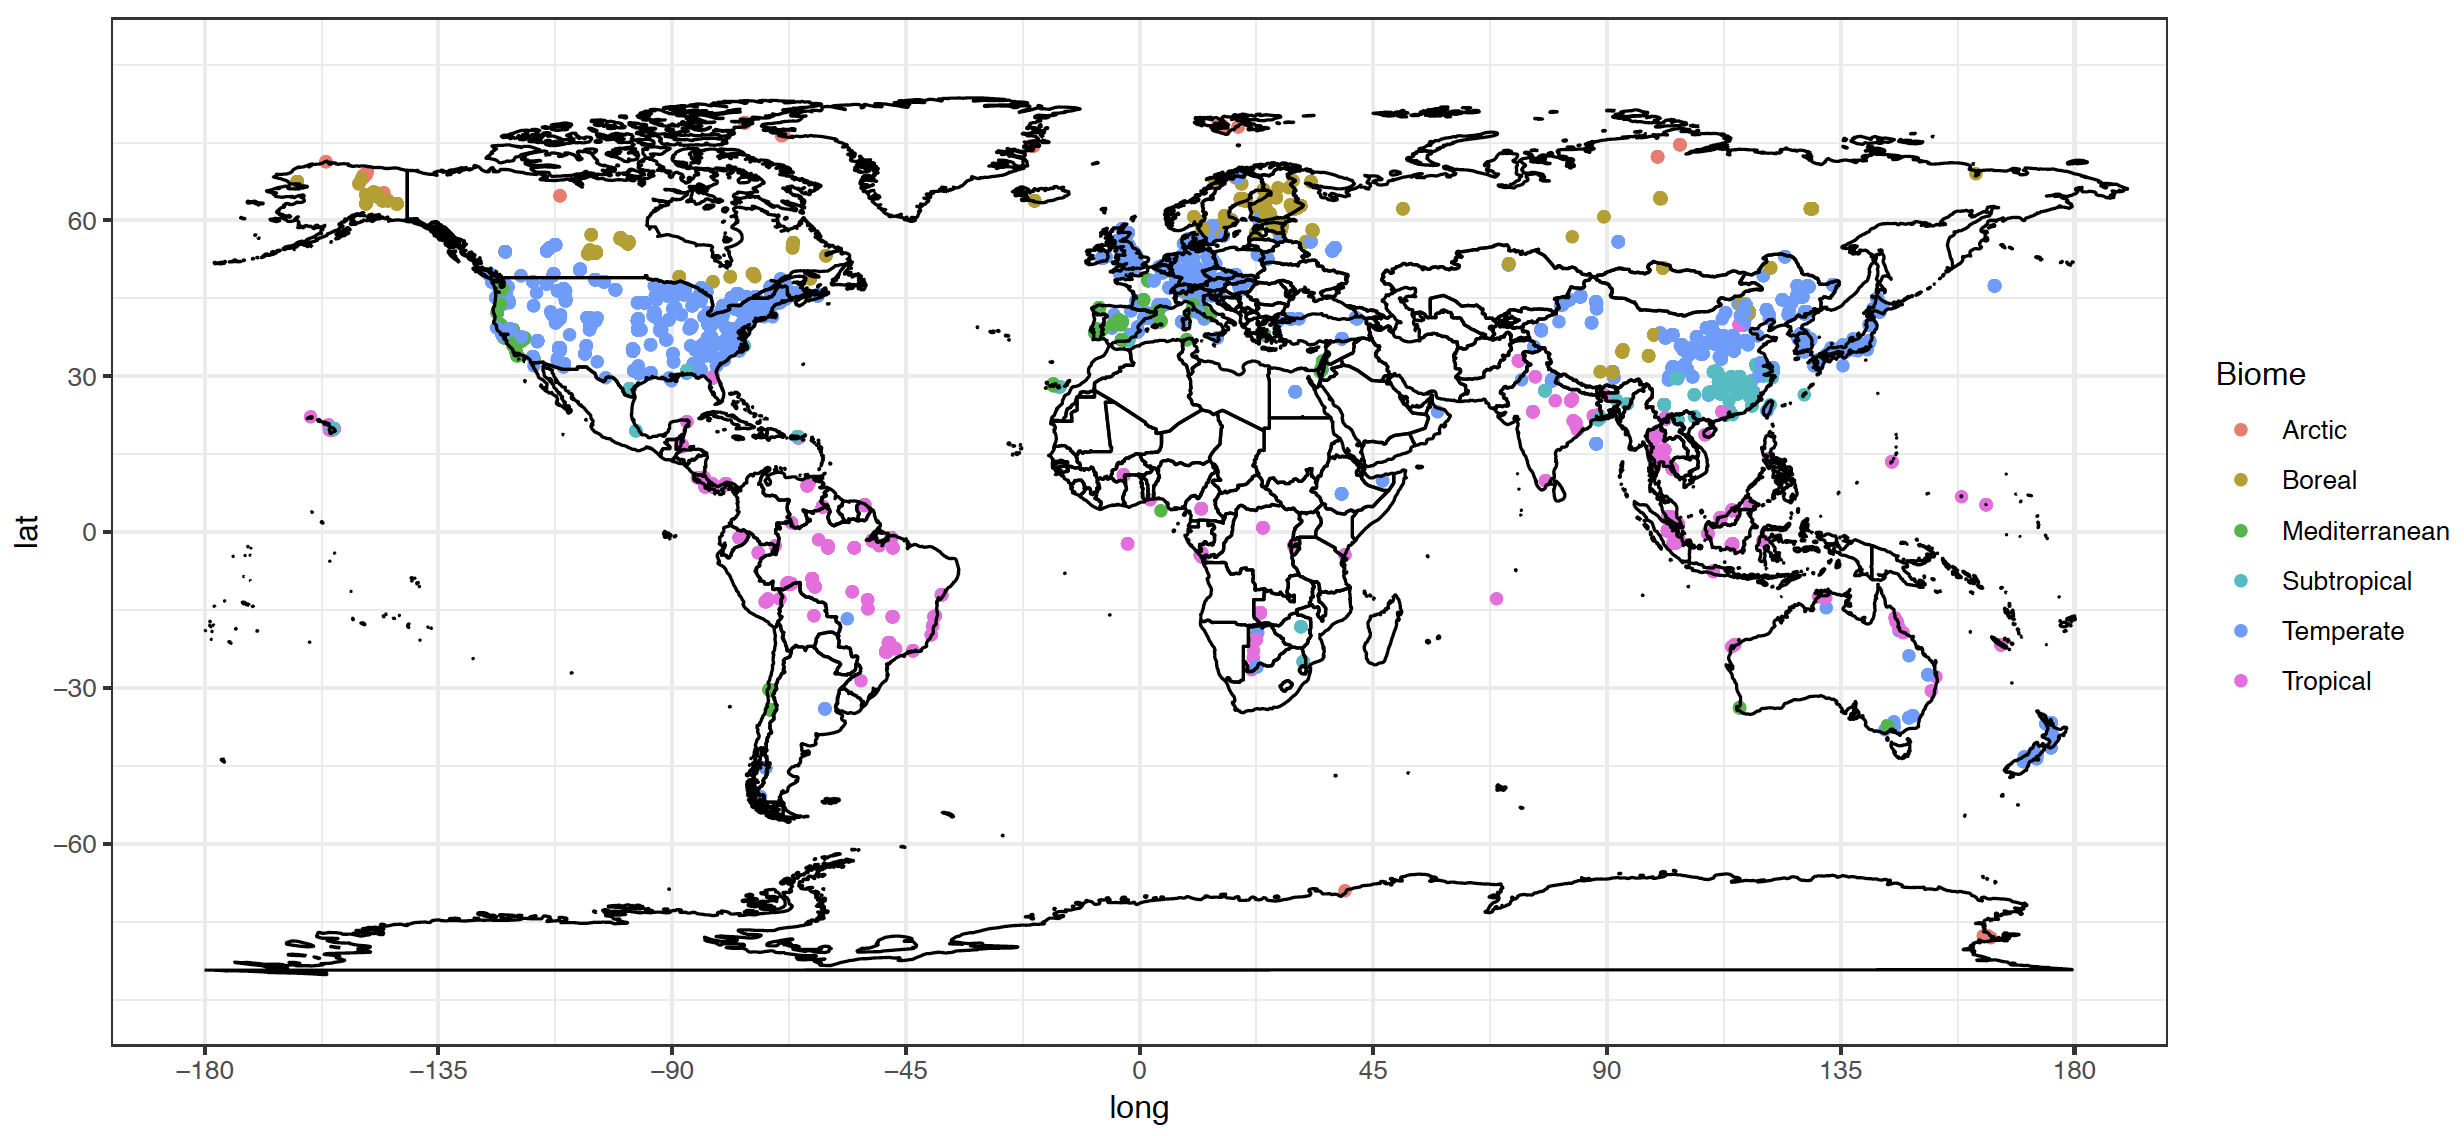
\includegraphics{SRDB_V4_Fig1.png}
\caption{Global spatial distribution of soil respiration sites}
\end{figure}

Rs data from cold regions are more important, but how to increase the
number of measurements? * Make equipment work normally in very cold and
remote conditions * Increase resources devoted to Rs measurements *
Methodological improvements: for instance, measuring once per day to get
daily mean

\begin{figure}
\centering
\includegraphics{Jessens.png}
\caption{Rs measured at diurnal soil temperature}
\end{figure}

\begin{itemize}
\tightlist
\item
  Measure once per year to get annual Rs mean? This is \textbf{Bahn's
  approach} \href{http://dx.doi.org/10.5194/bg-7-2147-2010}{Bahn et
  al.~(2004) Biogeosciences}
\end{itemize}

\begin{figure}
\centering
\includegraphics{Rs_MAT_Rs_Annual_Bahn2010.jpeg}
\caption{Rs measured at mean annual soil temperature}
\end{figure}

\begin{itemize}
\tightlist
\item
  Rs measured at annual mean temperature is \sout{linearly} related with
  annual Rs rate
\item
  Rs at mean temperature: soil respiration measured at annual mean
  temperature, monthly mean temperature, and/or daily mean temperature
\item
  \texttt{Rs\_annual} \textasciitilde{} \texttt{Rs\_mat} (``Rs\_bahn'')
\item
  \texttt{Rs\_annual} = 455.8 * \texttt{Rs\_mat}\^{}1.0054
  (R\textsuperscript{2} = 0.94, p\textless0.001)
\end{itemize}

\hypertarget{the-objects-of-this-analysis-are}{%
\section{2. The objects of this analysis
are}\label{the-objects-of-this-analysis-are}}

\begin{itemize}
\tightlist
\item
  Examine whether Rs measured at annual mean soil temperature can
  represent annual Rs rate? (We now have an order of magnitude more data
  than Bahn et al.)
\item
  Annual mean air temperature (e.g., average of 12 monthes' air
  temperature of 2000) / Mean annual air temperature (1964-2014)
\item
  If not, when and what is the mechanism?
\item
  Update the model?
\end{itemize}

\hypertarget{methods}{%
\section{3. Methods}\label{methods}}

\textbf{Data}

\begin{itemize}
\tightlist
\item
  Use SRDB\_V4 -- \texttt{Rs\_Annual}
\item
  Annual mean soil temperature (reported in the papers or can be
  calculated with simple assumptions)
\item
  Relationship between Rs and soil temperature (SRDB\_V4)
\item
  Air temperature (University of Daleware global precipitation and air
  temperature data, 1964-2014, half degree spatial resolusion)
\item
  823 records from 253 studies
\end{itemize}

\textbf{Statistics}

\begin{itemize}
\tightlist
\item
  According the the relationship between Rs and Ts, we can estimate
  \texttt{Rs\_mat} based on the annual mean soil temperature, T\_Annual,
  and/or MAT
\item
  Use the Bahn Biogeoscience model (Rs\_annual = 455.8 *
  Rs\_mat\^{}1.0054) to predict \texttt{Rs\_annual} based on
  \texttt{Rs\_mat}
\item
  Comparing \texttt{Rs\_annual} and \texttt{Rs\_annual\_bahn} to
  evaluate the performance of Bahn model across the global
\end{itemize}

\textbf{Update Bahn's model}

\begin{itemize}
\tightlist
\item
  If Bahn (2010) model does not predict Rs\_annual in all conditions
\item
  Update Bahn (2010) model (e.g., including drought parameter, other
  parameters?)
\item
  Regression tree modeling?
\end{itemize}

\includegraphics{6-Bahn_Analysis_Report_files/figure-latex/unnamed-chunk-2-1.pdf}

\hypertarget{test-the-relationship-between-rs_annual-and-rs_mat}{%
\subsection{3.2 test the relationship between Rs\_annual and
Rs\_mat}\label{test-the-relationship-between-rs_annual-and-rs_mat}}

\begin{verbatim}
## Wed Apr  3 14:31:54 2019  -------------------
## Wed Apr  3 14:31:54 2019  Bahn relationship for these data:
## 
## Call:
## lm(formula = Rs_TAIR ~ Rs_annual, data = sdata)
## 
## Residuals:
##      Min       1Q   Median       3Q      Max 
## -1006.45   -84.72    14.90    93.38   964.58 
## 
## Coefficients:
##             Estimate Std. Error t value Pr(>|t|)    
## (Intercept)  0.64266   13.67584   0.047    0.963    
## Rs_annual    0.85184    0.01466  58.126   <2e-16 ***
## ---
## Signif. codes:  0 '***' 0.001 '**' 0.01 '*' 0.05 '.' 0.1 ' ' 1
## 
## Residual standard error: 185.1 on 821 degrees of freedom
## Multiple R-squared:  0.8045, Adjusted R-squared:  0.8043 
## F-statistic:  3379 on 1 and 821 DF,  p-value: < 2.2e-16
\end{verbatim}

\includegraphics{6-Bahn_Analysis_Report_files/figure-latex/unnamed-chunk-3-1.pdf}

\begin{verbatim}
## [1] "test intercept=0 and slope=1"
## [1] "p_intercept = 0.9625, p_slope = 0"
\end{verbatim}

\hypertarget{ts-sources-mgrsd-mgrsd_tair-from-paper-rs_ts_relationship}{%
\subsection{3.3 Ts sources (MGRsD, MGRsD\_TAIR, From paper,
Rs\_Ts\_relationship)}\label{ts-sources-mgrsd-mgrsd_tair-from-paper-rs_ts_relationship}}

\begin{verbatim}
## Saving 7 x 5 in image
\end{verbatim}

\includegraphics{6-Bahn_Analysis_Report_files/figure-latex/unnamed-chunk-4-1.pdf}

\hypertarget{annual-rs-or-ts-coverage-effect}{%
\subsection{3.4 Annual Rs or Ts coverage
effect}\label{annual-rs-or-ts-coverage-effect}}

\begin{verbatim}
## Saving 7 x 5 in image
\end{verbatim}

\includegraphics{6-Bahn_Analysis_Report_files/figure-latex/unnamed-chunk-5-1.pdf}

\begin{verbatim}
## Saving 7 x 5 in image
\end{verbatim}

\includegraphics{6-Bahn_Analysis_Report_files/figure-latex/unnamed-chunk-5-2.pdf}

\hypertarget{test-whether-outliers-affect-the-regression-need-update}{%
\subsection{3.4.1 Test whether outliers affect the regression (need
update)}\label{test-whether-outliers-affect-the-regression-need-update}}

\begin{itemize}
\tightlist
\item
  Conclusion: need to update the code and results
\end{itemize}

\begin{verbatim}
## Saving 7 x 5 in image
\end{verbatim}

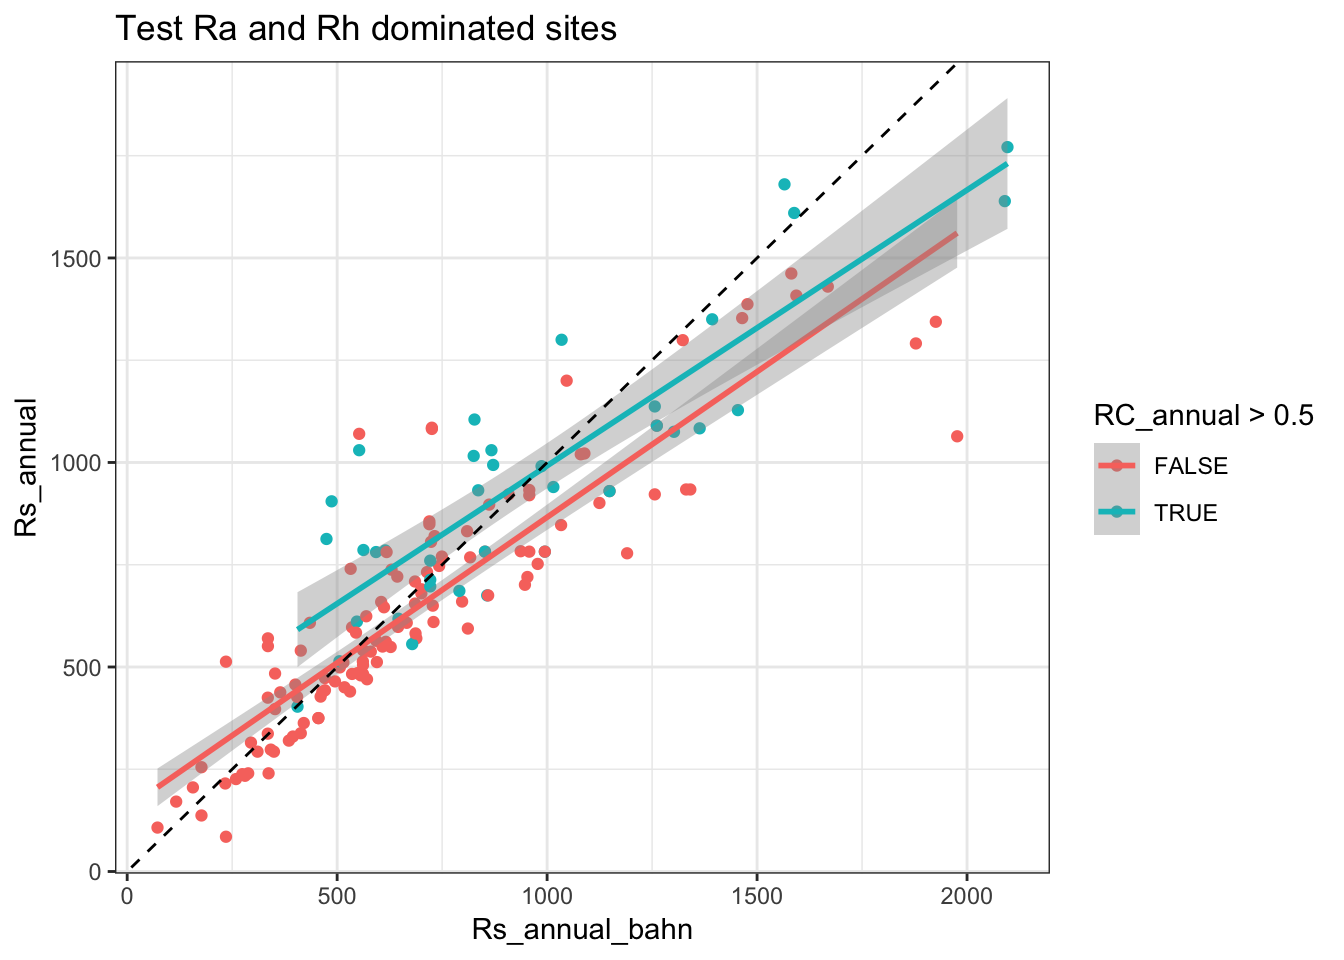
\includegraphics{6-Bahn_Analysis_Report_files/figure-latex/unnamed-chunk-6-1.pdf}

\begin{verbatim}
## Saving 7 x 5 in image
\end{verbatim}

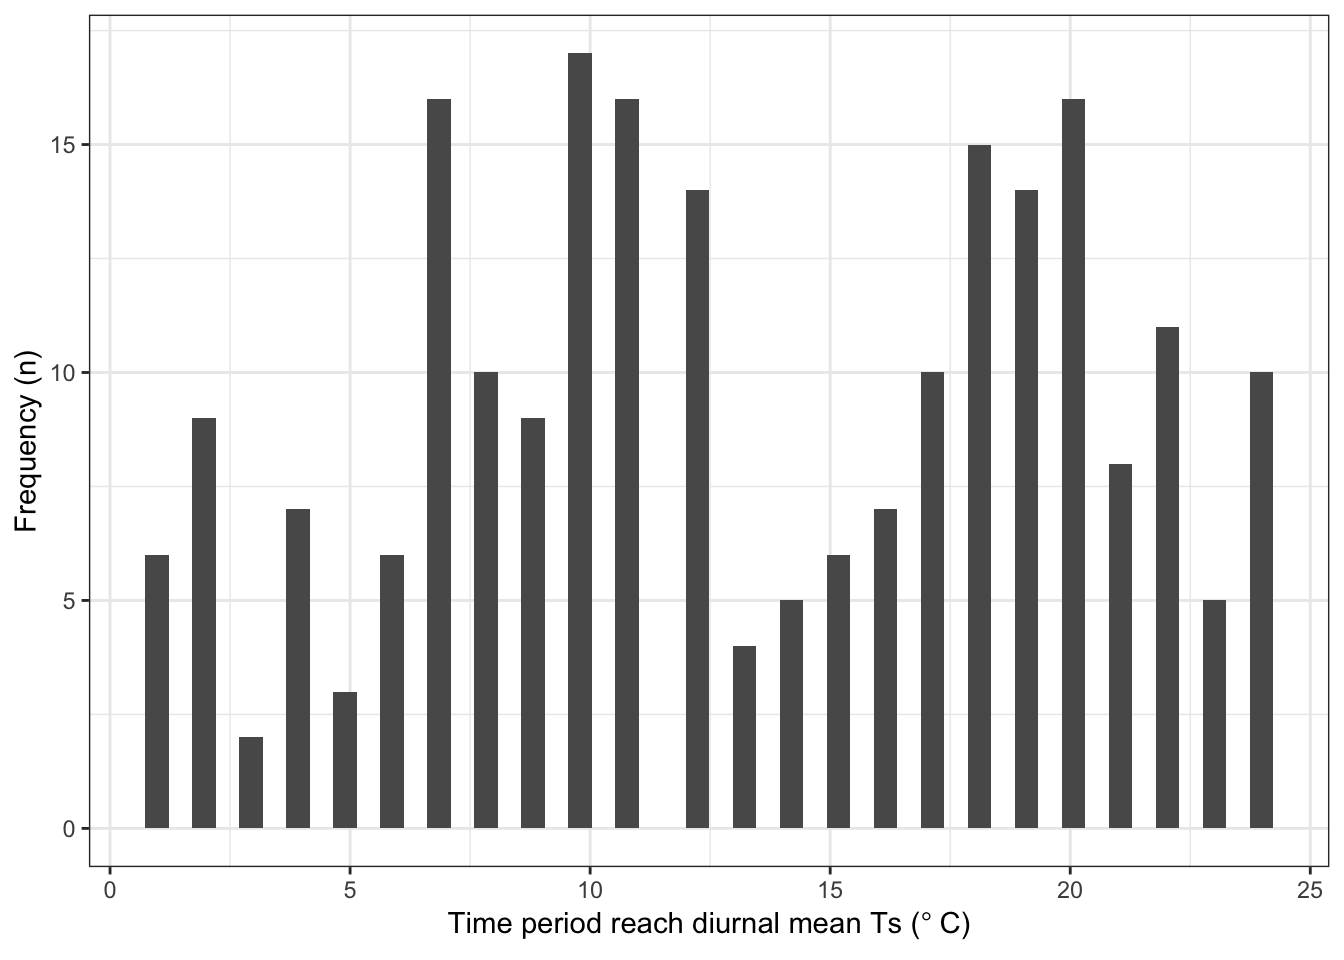
\includegraphics{6-Bahn_Analysis_Report_files/figure-latex/unnamed-chunk-6-2.pdf}

\hypertarget{effect-of-maximum-allowed-divergence-between-global-climate-data-set-and-site-specific-air-temperature}{%
\subsection{3.4.2 Effect of maximum allowed divergence between global
climate data set and site-specific air
temperature}\label{effect-of-maximum-allowed-divergence-between-global-climate-data-set-and-site-specific-air-temperature}}

\begin{itemize}
\tightlist
\item
  Does TAIR\_dev and TAIR\_LT\textless\_dev affect the relationship --
  YES!!!!!
\item
  TAIR\_LTM\_dev = with( srdb, abs( MAT\_Del - MAT ) )
\item
  Does TAIR\_LTM\_dev () pull the slope off 1? -- YES!!!!!
\item
  TAIR\_dev \textless- with( srdb, abs( TAnnual\_Del - Study\_temp ) )
\item
  Figure E. Effect of maximum allowed divergence between global climate
  data set and site-specific air temperature, when given. As we throw
  out data points with high divergence, R2 goes up (top panel) and RSE
  goes down (bottom, g C m-2 yr-1).
\end{itemize}

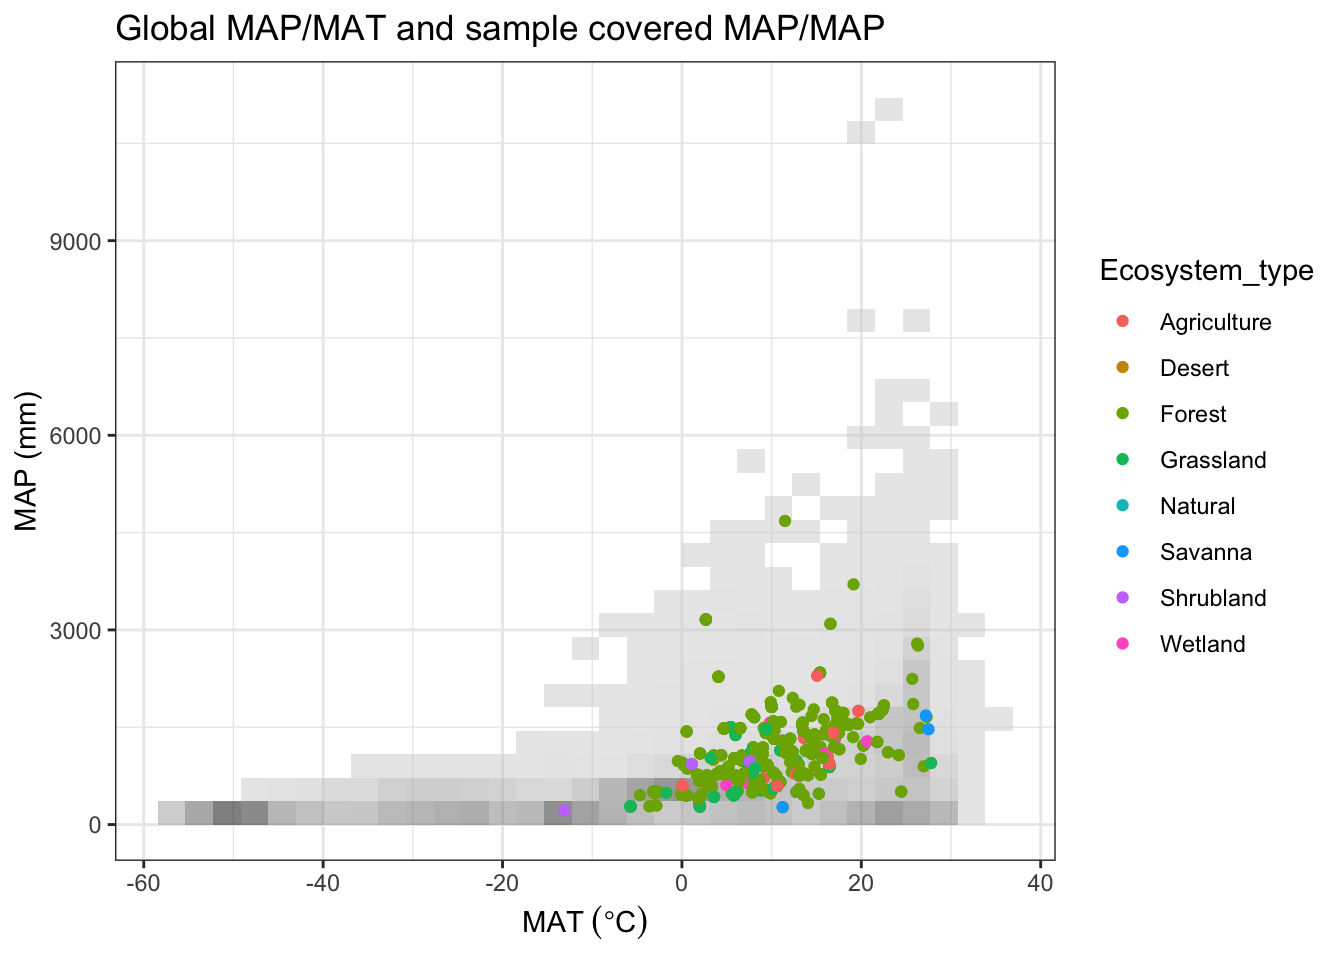
\includegraphics{6-Bahn_Analysis_Report_files/figure-latex/unnamed-chunk-7-1.pdf}

\begin{verbatim}
## Saving 7 x 5 in image
\end{verbatim}

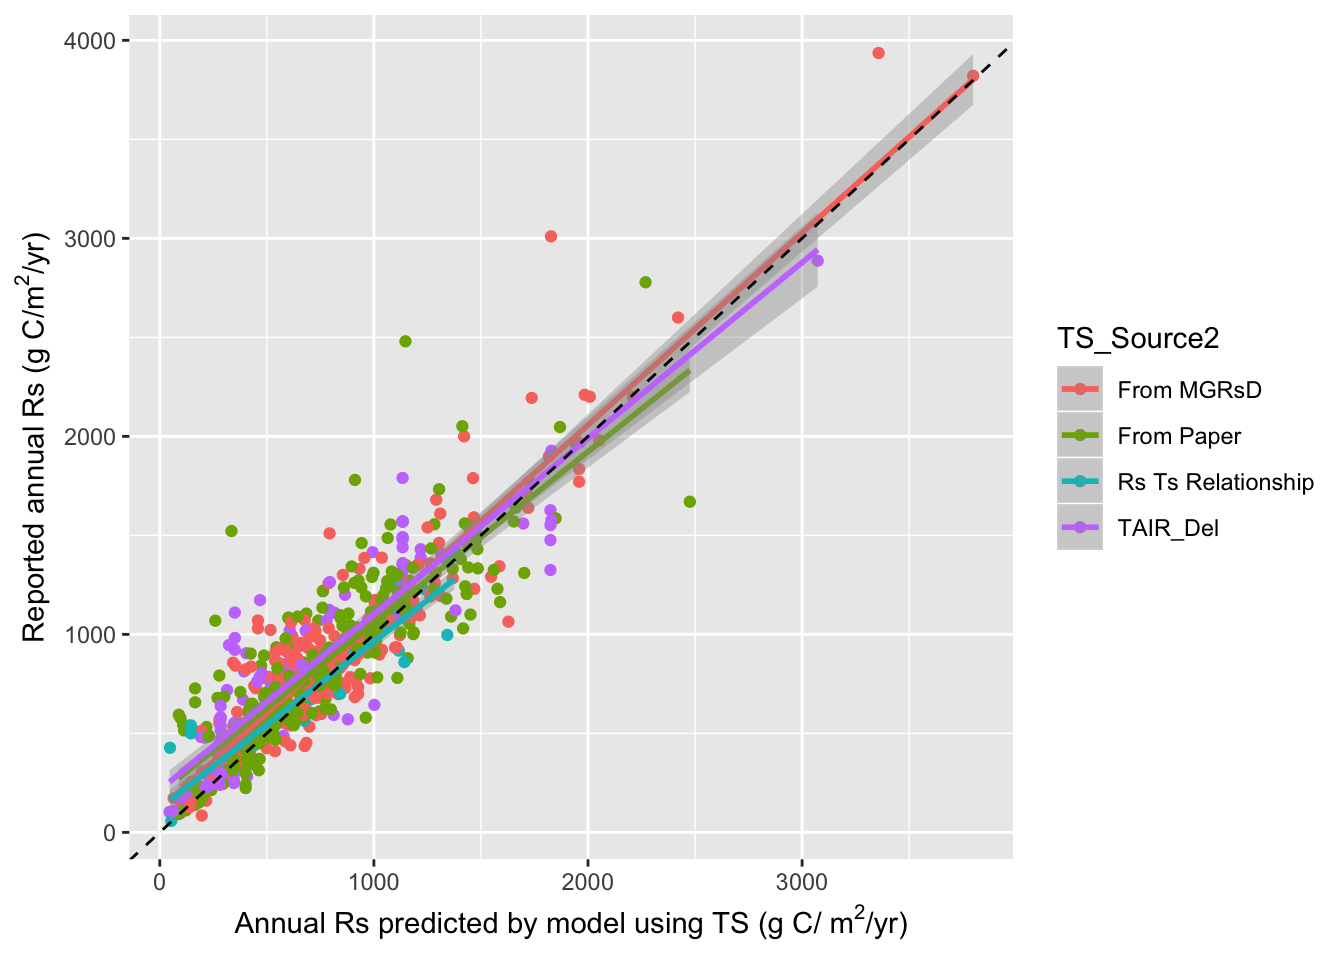
\includegraphics{6-Bahn_Analysis_Report_files/figure-latex/unnamed-chunk-8-1.pdf}

\begin{verbatim}
## Saving 7 x 5 in image
\end{verbatim}

\includegraphics{6-Bahn_Analysis_Report_files/figure-latex/unnamed-chunk-8-2.pdf}

\hypertarget{effect-of-maximum-allowed-divergence-between-annual-precipitation-from-paper-and-del}{%
\subsection{3.4.3 Effect of maximum allowed divergence between annual
precipitation from paper and
Del}\label{effect-of-maximum-allowed-divergence-between-annual-precipitation-from-paper-and-del}}

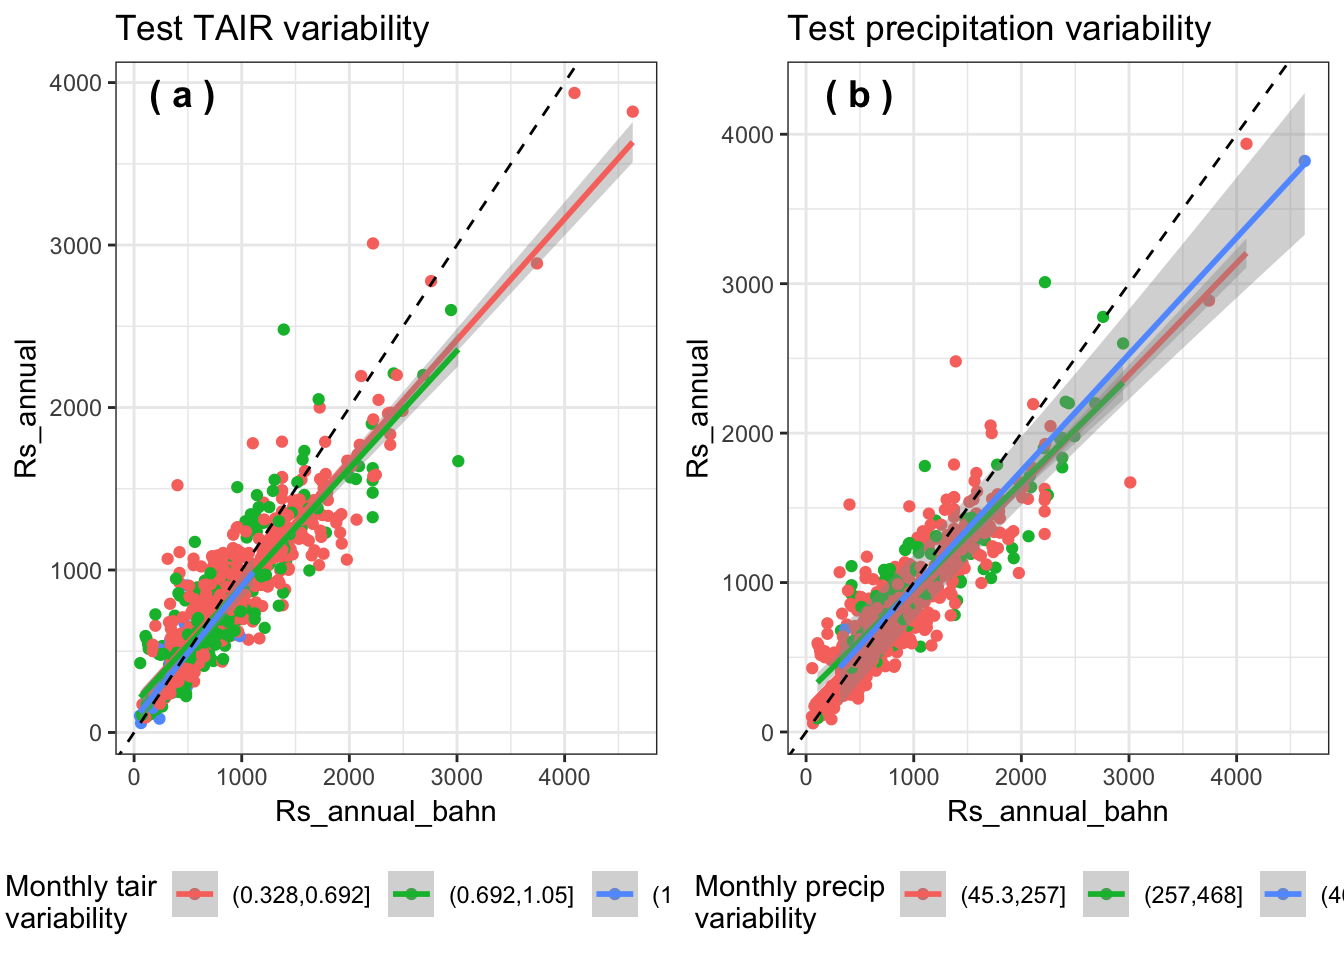
\includegraphics{6-Bahn_Analysis_Report_files/figure-latex/unnamed-chunk-9-1.pdf}

\hypertarget{results}{%
\section{4. Results}\label{results}}

\hypertarget{using-ts-tannual-or-mat}{%
\subsection{4.1 Using Ts, TAnnual or
MAT}\label{using-ts-tannual-or-mat}}

\hypertarget{using-soil-temperature}{%
\subsubsection{4.1.1 Using soil
temperature}\label{using-soil-temperature}}

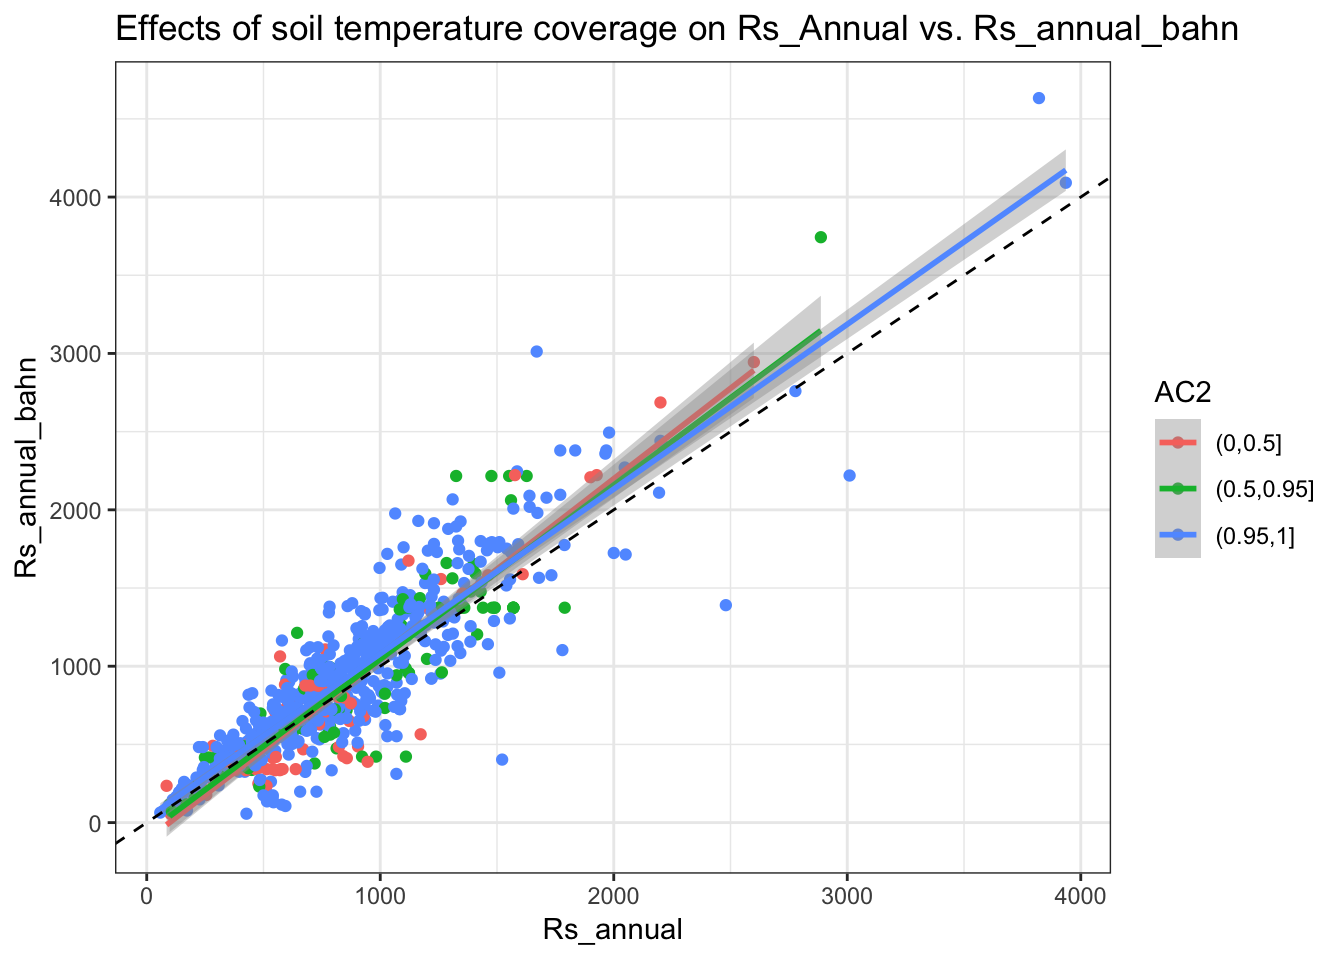
\includegraphics{6-Bahn_Analysis_Report_files/figure-latex/unnamed-chunk-10-1.pdf}

\begin{verbatim}
## Saving 7 x 5 in image
\end{verbatim}

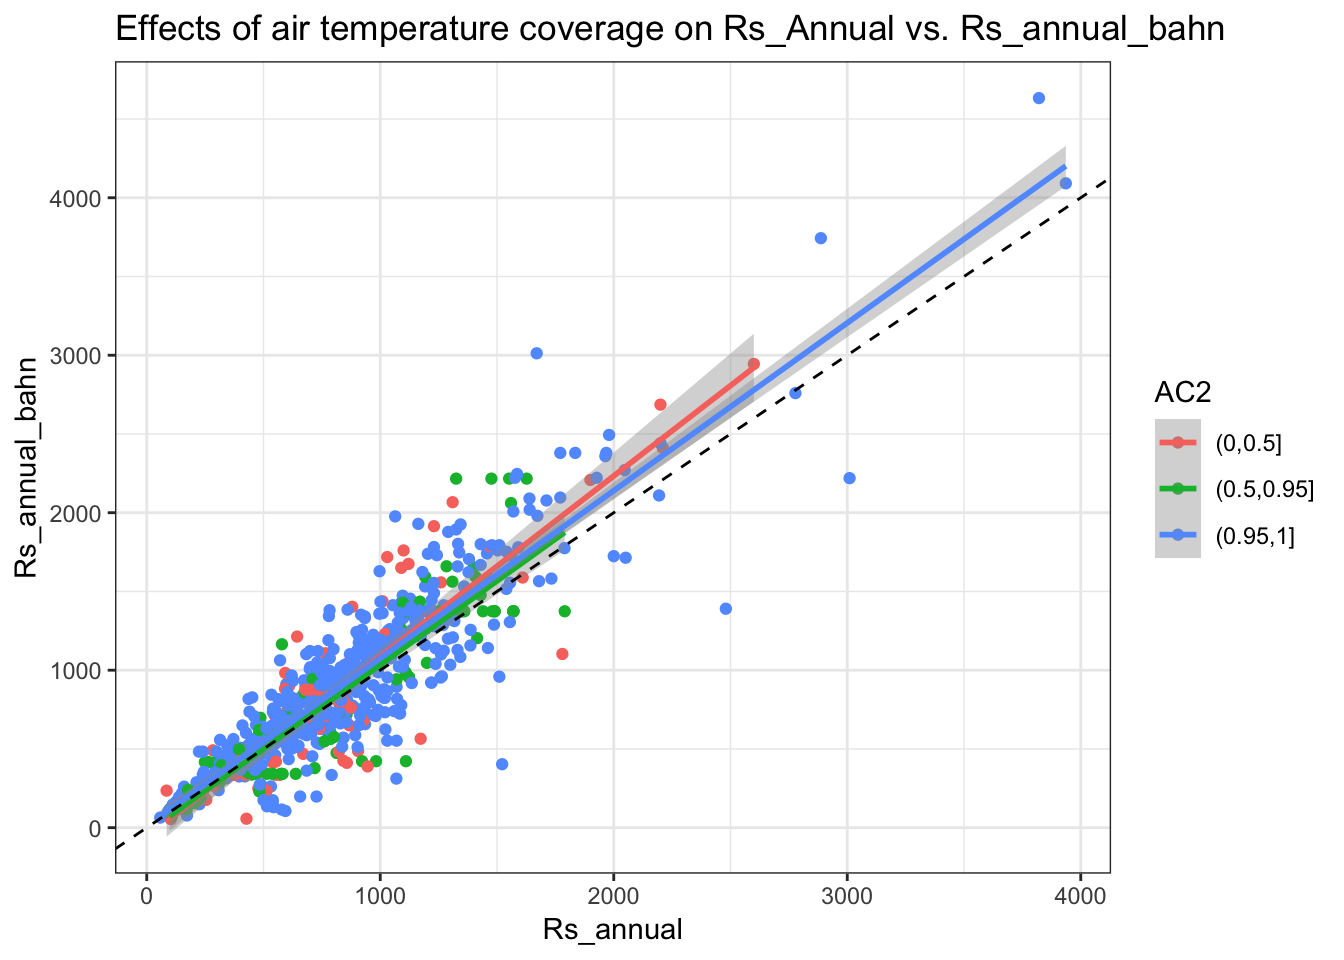
\includegraphics{6-Bahn_Analysis_Report_files/figure-latex/unnamed-chunk-10-2.pdf}

\hypertarget{using-t_annual}{%
\subsubsection{4.1.2 Using T\_Annual}\label{using-t_annual}}

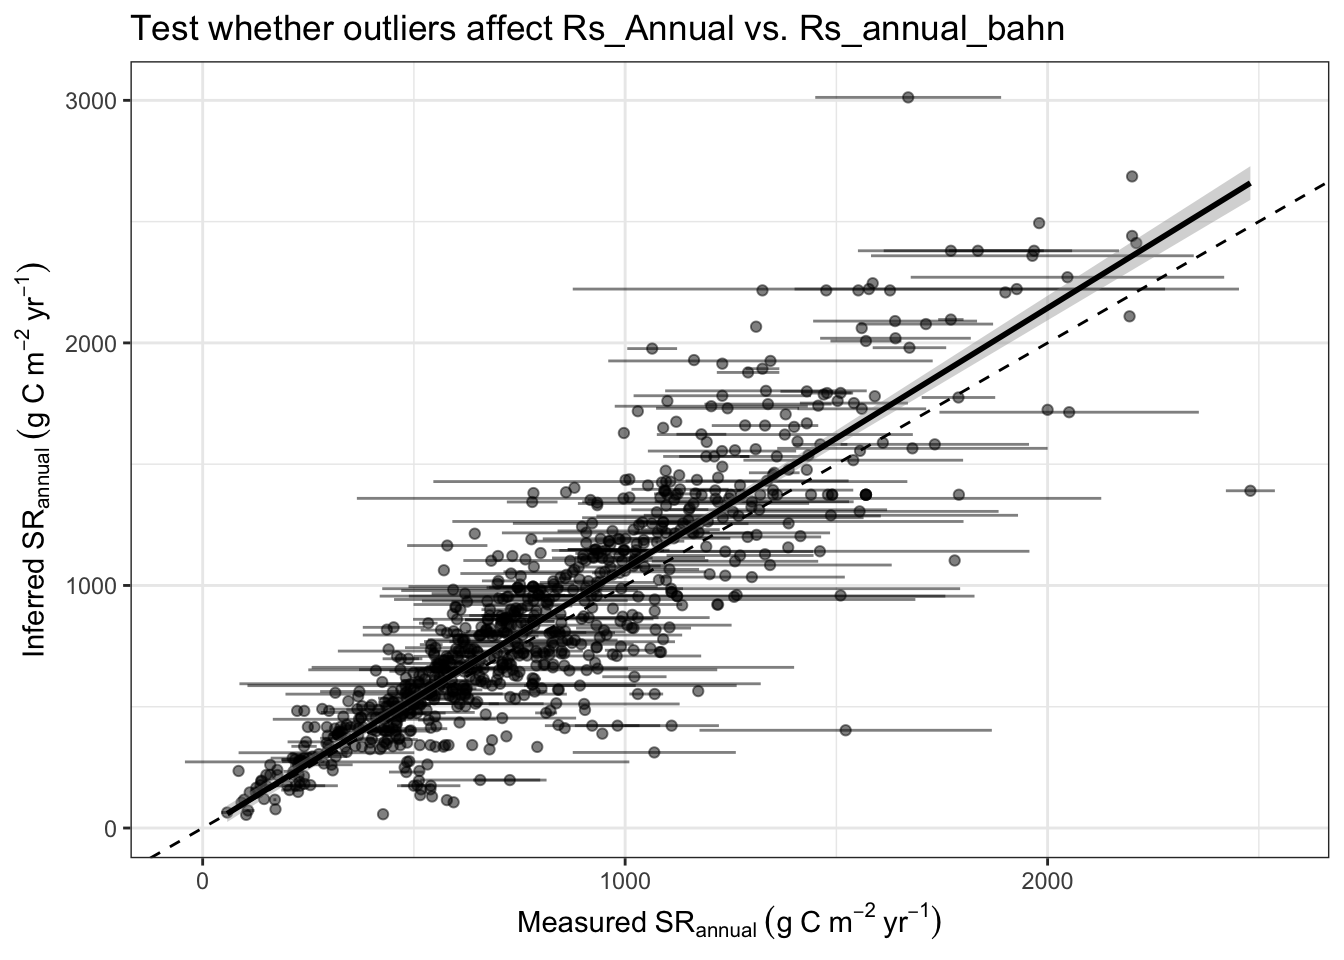
\includegraphics{6-Bahn_Analysis_Report_files/figure-latex/unnamed-chunk-11-1.pdf}

\begin{verbatim}
## Saving 7 x 5 in image
\end{verbatim}

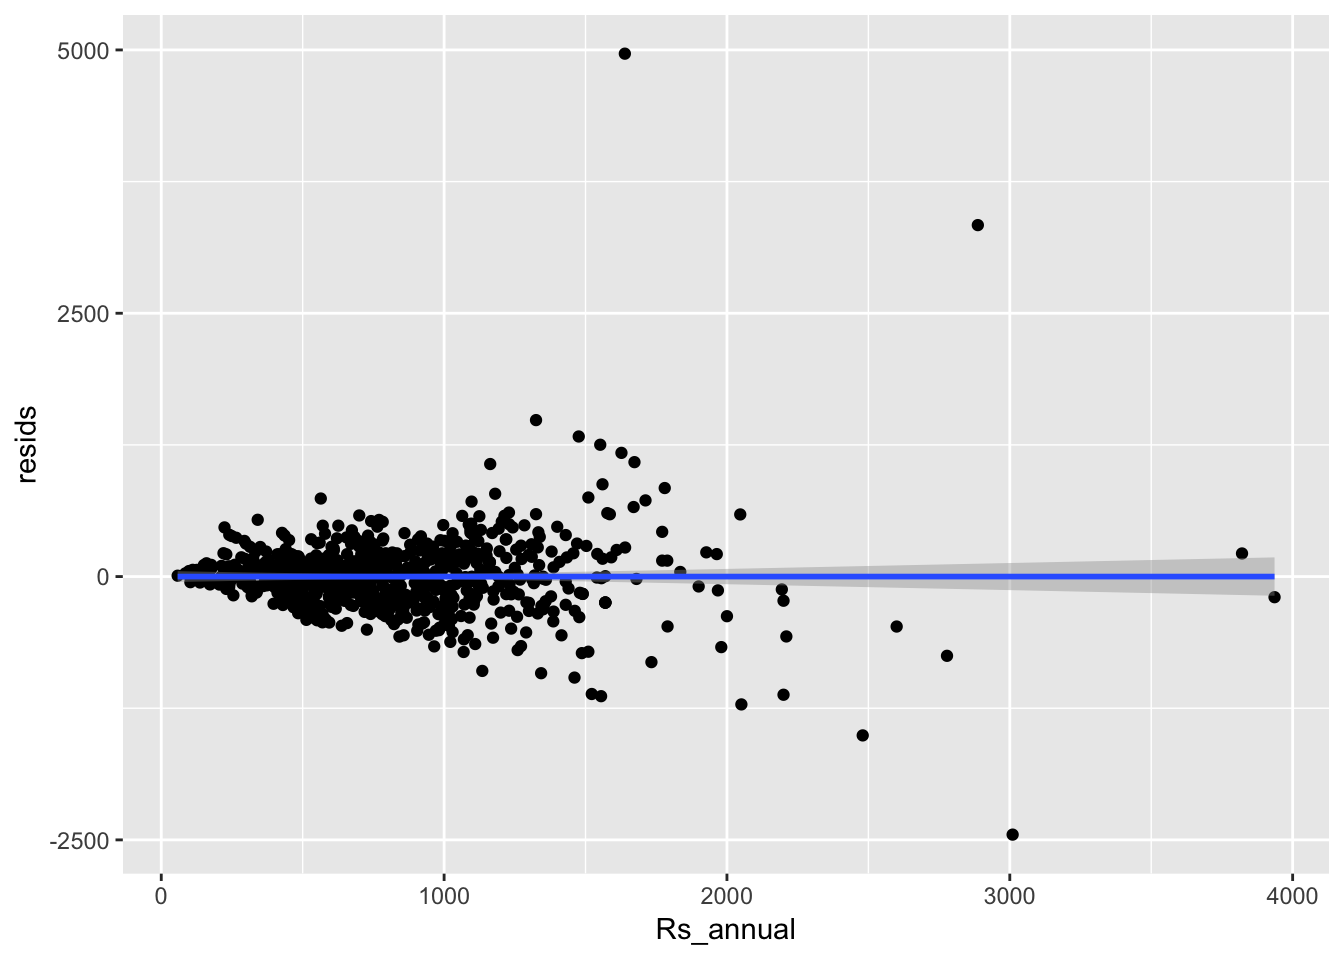
\includegraphics{6-Bahn_Analysis_Report_files/figure-latex/unnamed-chunk-11-2.pdf}

\hypertarget{using-mat}{%
\subsubsection{4.1.3 Using MAT}\label{using-mat}}

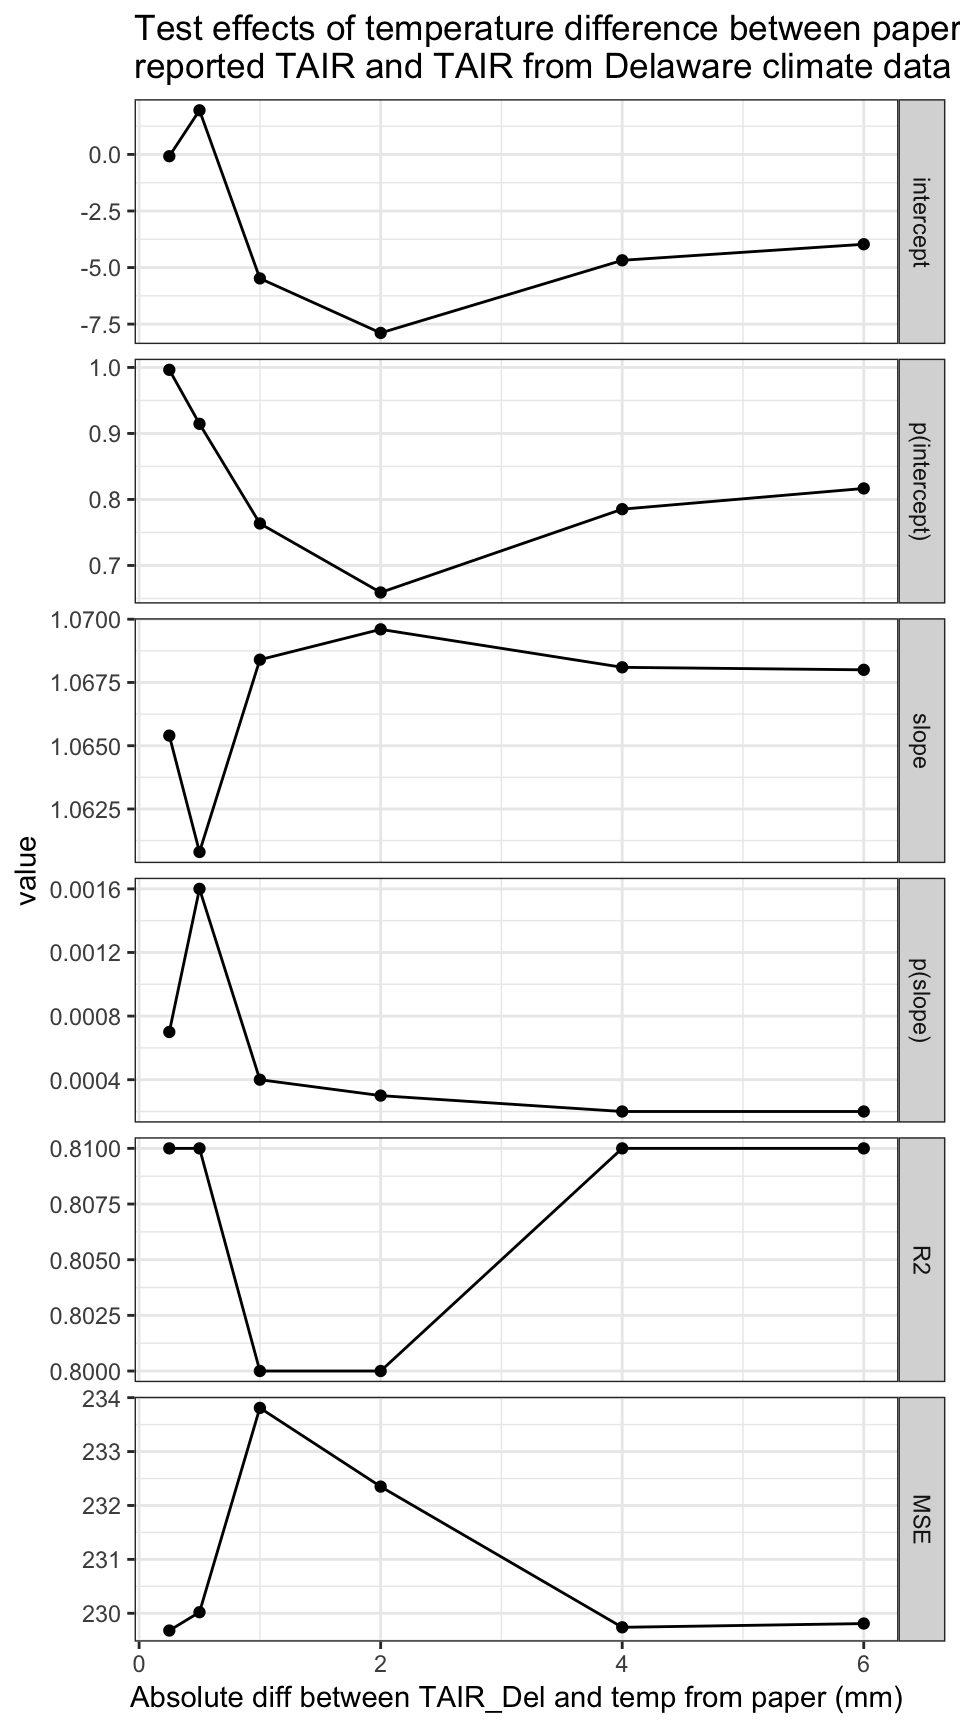
\includegraphics{6-Bahn_Analysis_Report_files/figure-latex/unnamed-chunk-12-1.pdf}

\begin{verbatim}
## Saving 7 x 5 in image
\end{verbatim}

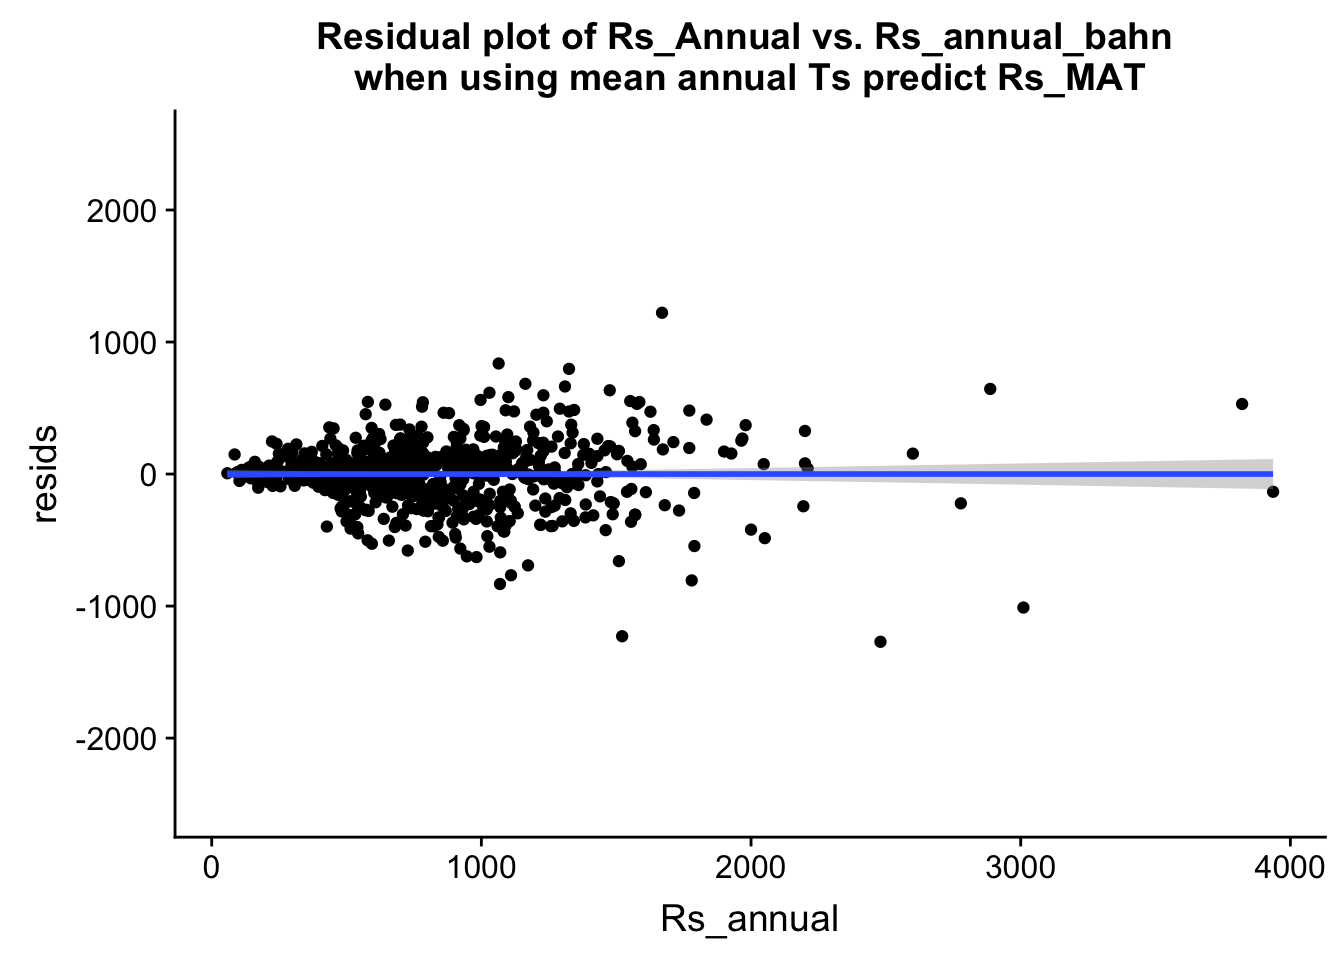
\includegraphics{6-Bahn_Analysis_Report_files/figure-latex/unnamed-chunk-12-2.pdf}

\hypertarget{analysis-when-rs_mat-cannot-represent-rs_annual}{%
\subsection{4.2 Analysis when Rs\_mat cannot represent
Rs\_annual}\label{analysis-when-rs_mat-cannot-represent-rs_annual}}

\hypertarget{does-ecosystem_type-affect-the-relationship-between-rs_annual-and-rs_mat}{%
\subsection{4.2.2 Does Ecosystem\_type affect the relationship between
Rs\_annual and
Rs\_mat?}\label{does-ecosystem_type-affect-the-relationship-between-rs_annual-and-rs_mat}}

\begin{verbatim}
## geom_path: Each group consists of only one observation. Do you need to
## adjust the group aesthetic?
## geom_path: Each group consists of only one observation. Do you need to
## adjust the group aesthetic?
## geom_path: Each group consists of only one observation. Do you need to
## adjust the group aesthetic?
## geom_path: Each group consists of only one observation. Do you need to
## adjust the group aesthetic?
## geom_path: Each group consists of only one observation. Do you need to
## adjust the group aesthetic?
## geom_path: Each group consists of only one observation. Do you need to
## adjust the group aesthetic?
\end{verbatim}

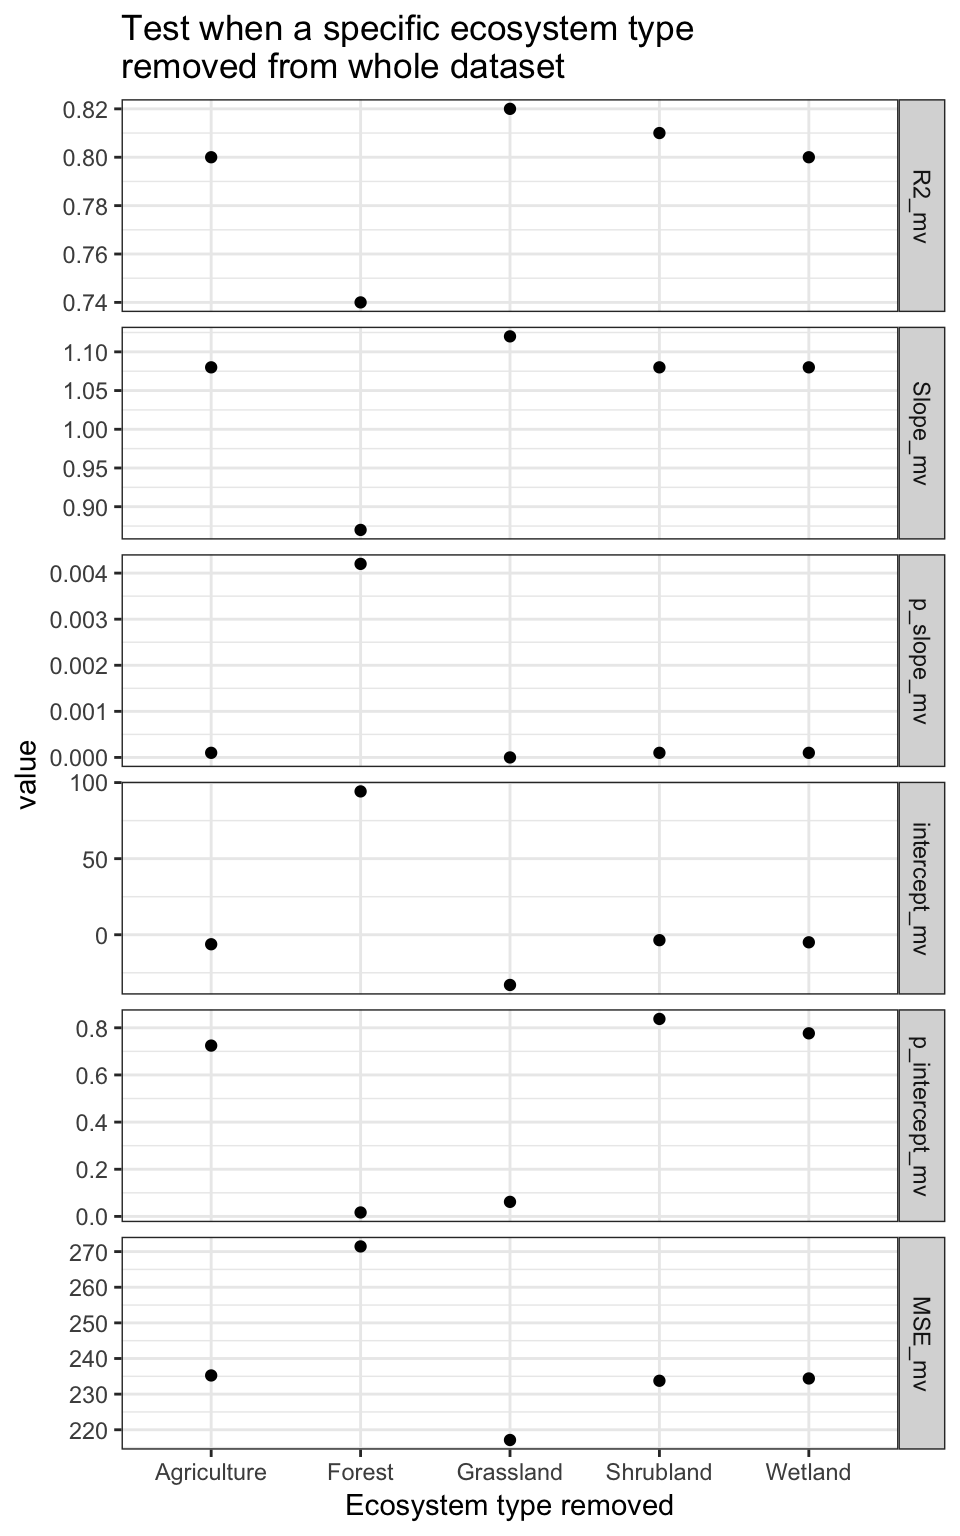
\includegraphics{6-Bahn_Analysis_Report_files/figure-latex/filtration_mk-1.pdf}

\begin{verbatim}
## geom_path: Each group consists of only one observation. Do you need to
## adjust the group aesthetic?
## geom_path: Each group consists of only one observation. Do you need to
## adjust the group aesthetic?
## geom_path: Each group consists of only one observation. Do you need to
## adjust the group aesthetic?
## geom_path: Each group consists of only one observation. Do you need to
## adjust the group aesthetic?
## geom_path: Each group consists of only one observation. Do you need to
## adjust the group aesthetic?
## geom_path: Each group consists of only one observation. Do you need to
## adjust the group aesthetic?
\end{verbatim}

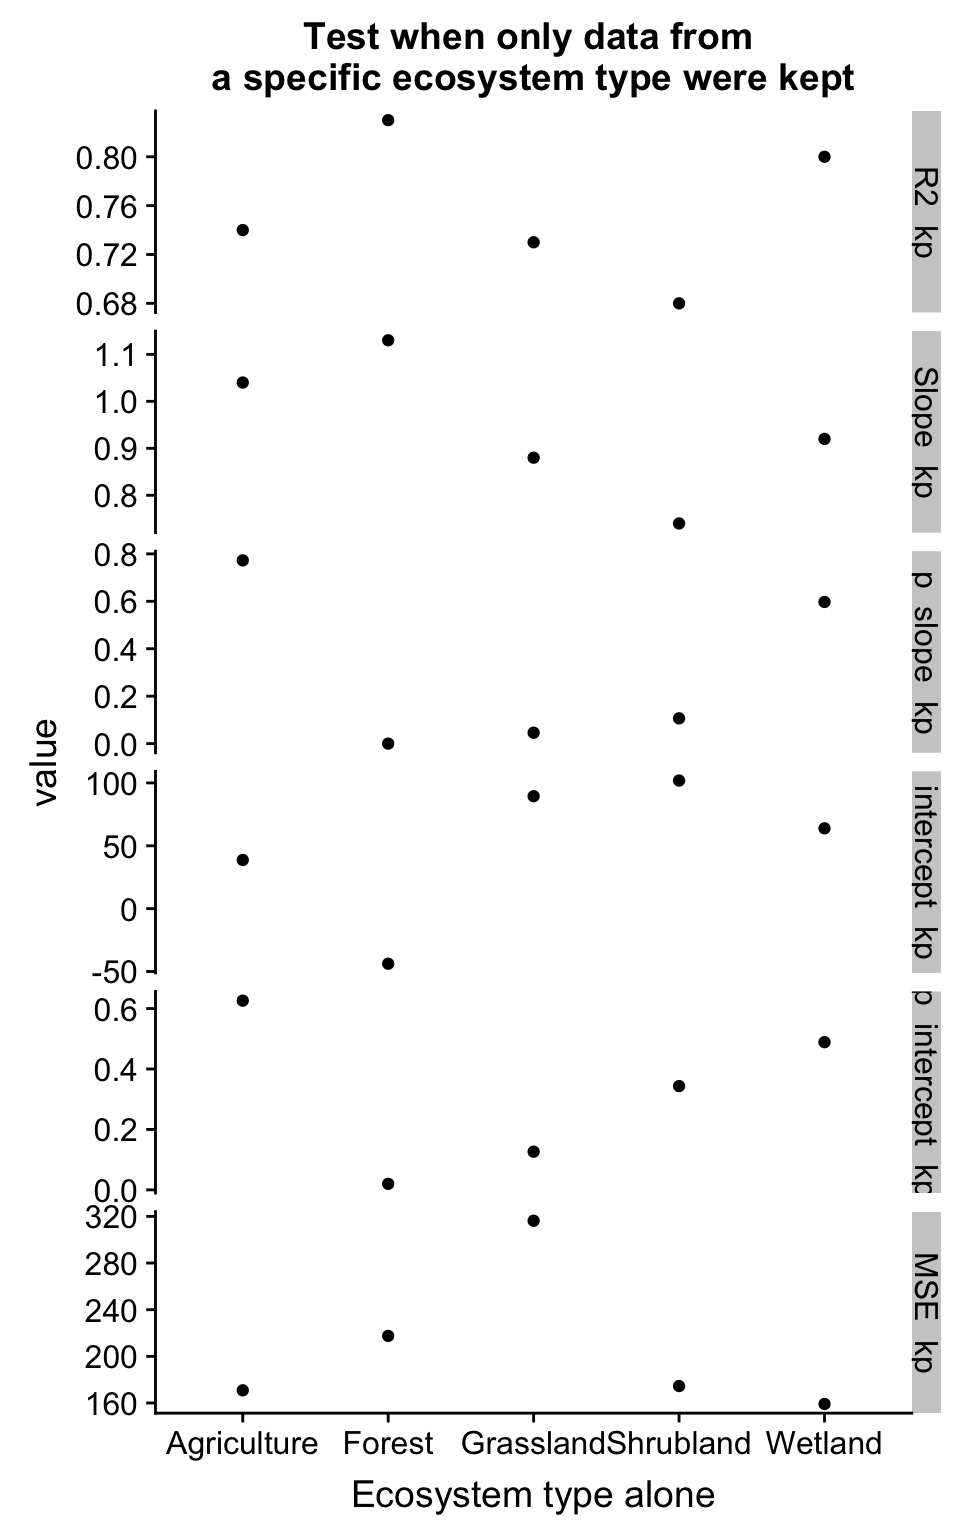
\includegraphics{6-Bahn_Analysis_Report_files/figure-latex/filtration_mk-2.pdf}

\begin{verbatim}
## Saving 7 x 5 in image
\end{verbatim}

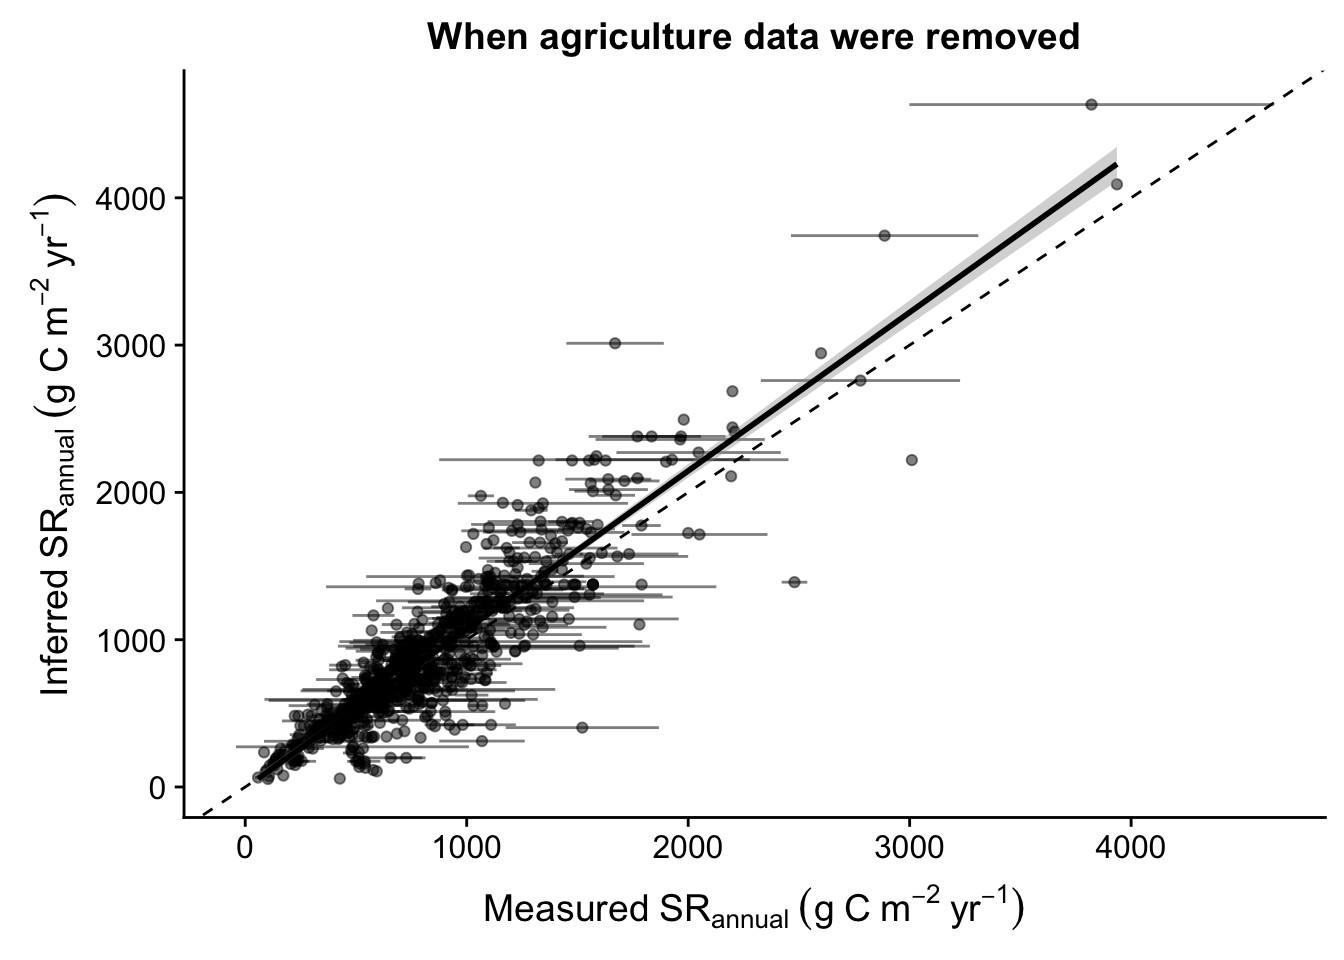
\includegraphics{6-Bahn_Analysis_Report_files/figure-latex/agriculture-1.pdf}

\begin{verbatim}
## Saving 7 x 5 in image
\end{verbatim}

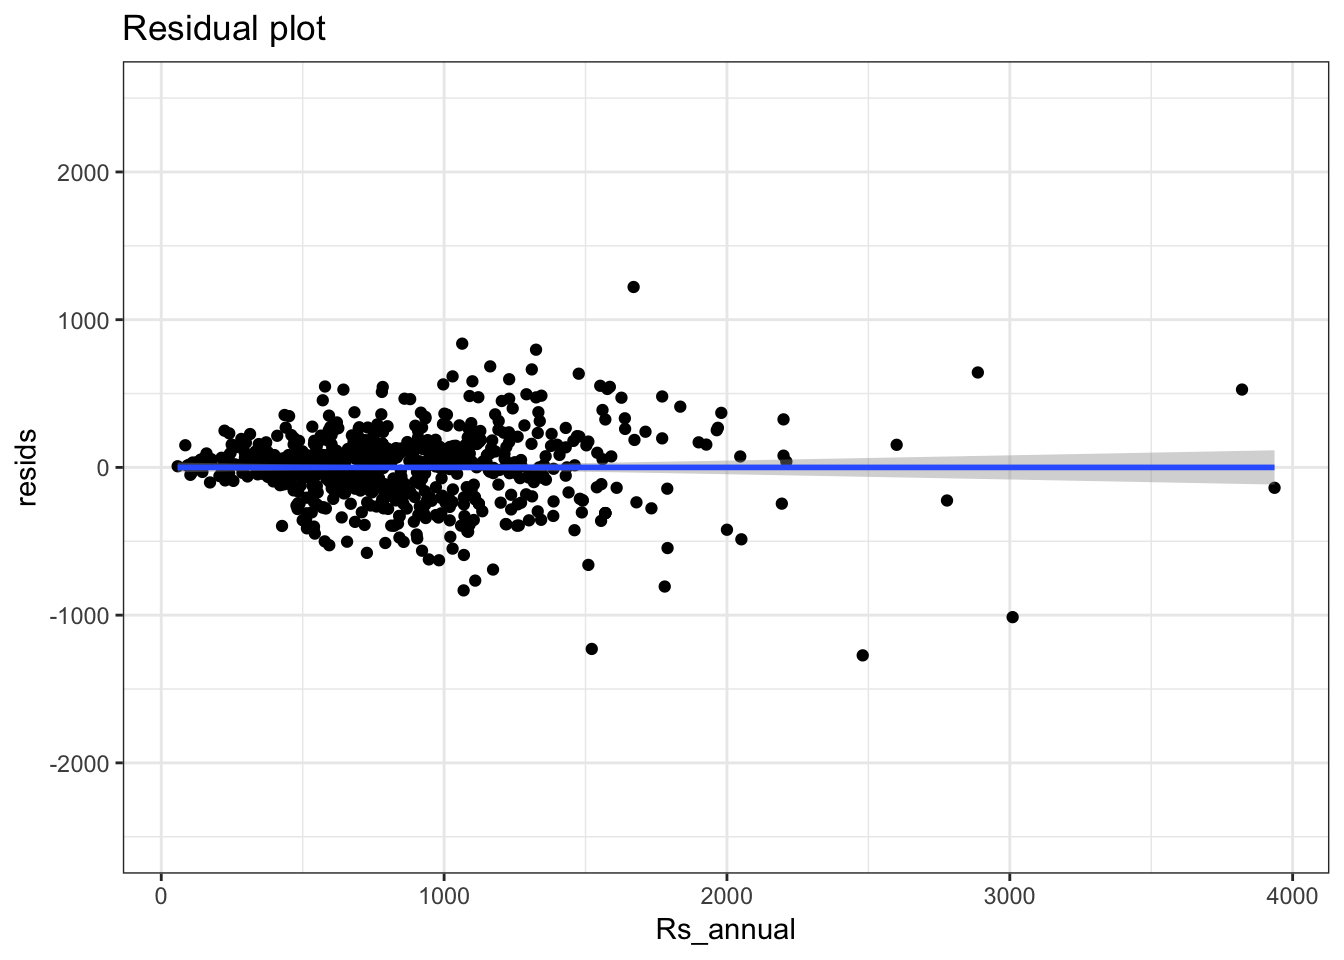
\includegraphics{6-Bahn_Analysis_Report_files/figure-latex/agriculture-2.pdf}

\begin{verbatim}
## Saving 7 x 5 in image
\end{verbatim}

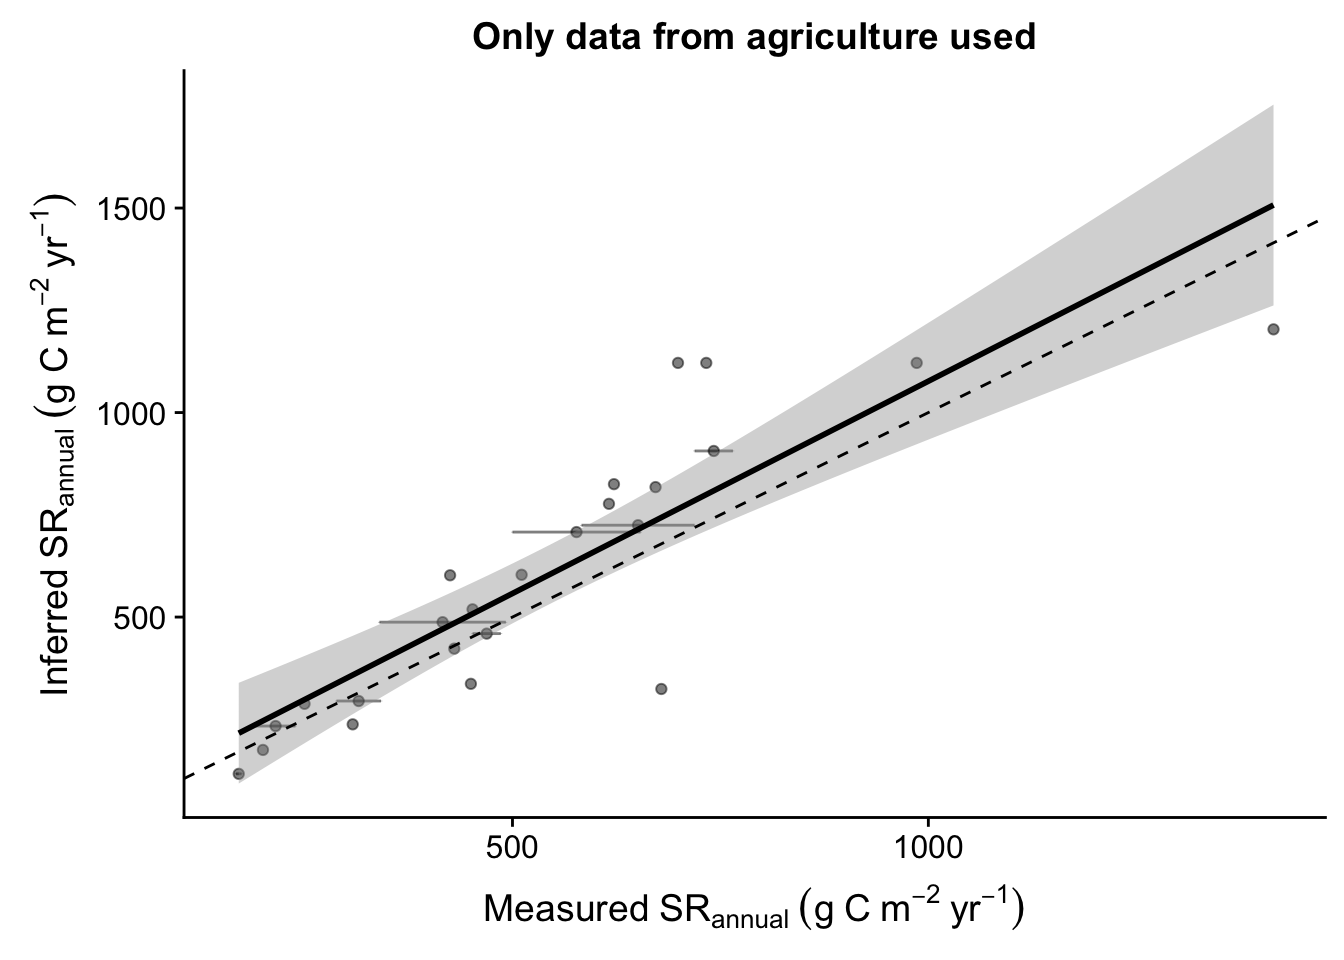
\includegraphics{6-Bahn_Analysis_Report_files/figure-latex/agriculture-3.pdf}

\begin{verbatim}
## Saving 7 x 5 in image
\end{verbatim}

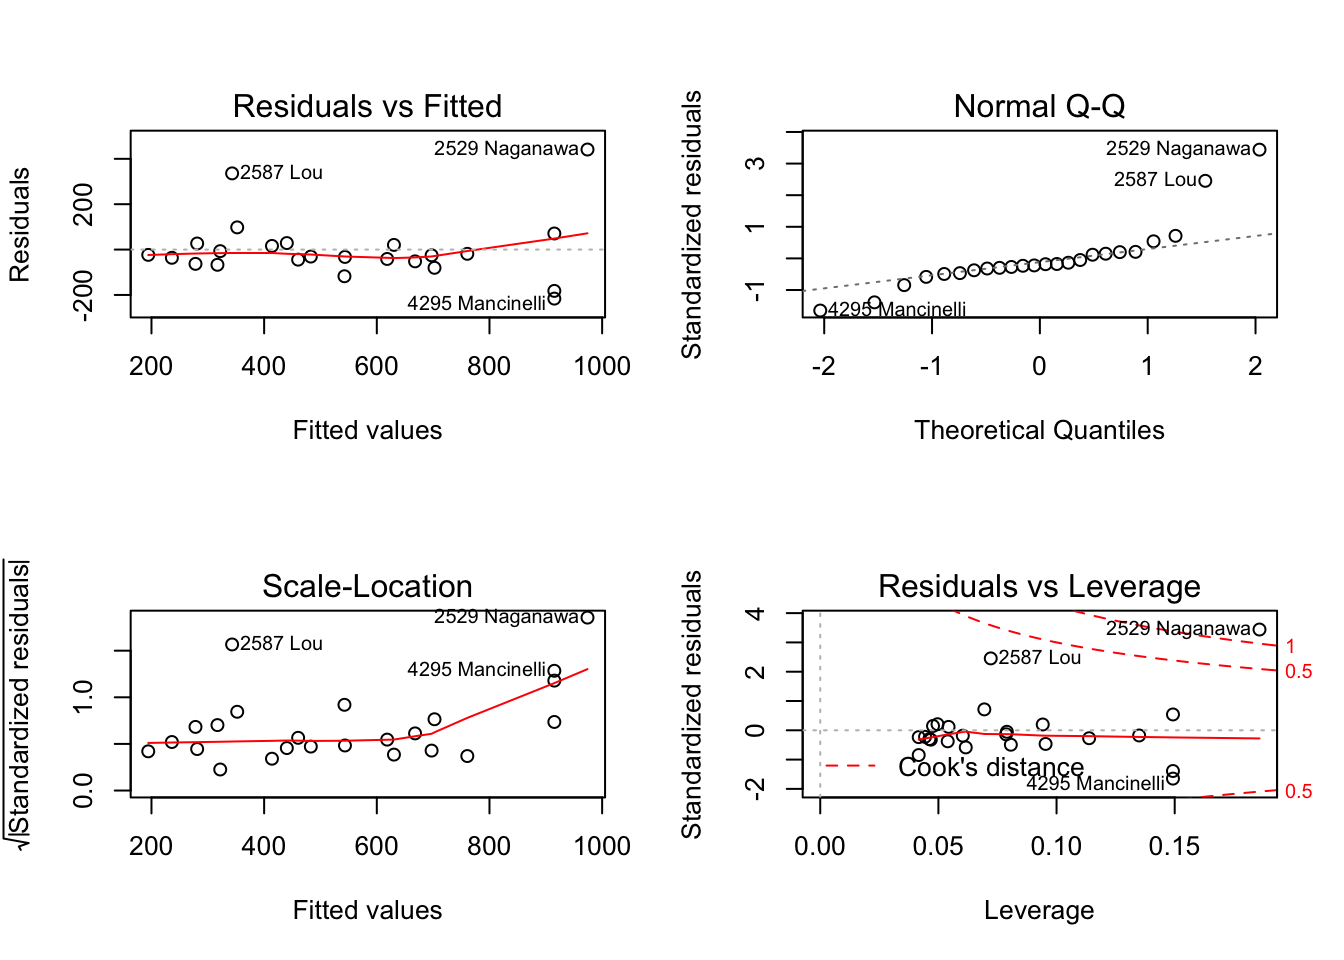
\includegraphics{6-Bahn_Analysis_Report_files/figure-latex/agriculture-4.pdf}

\begin{verbatim}
## Saving 7 x 5 in image
\end{verbatim}

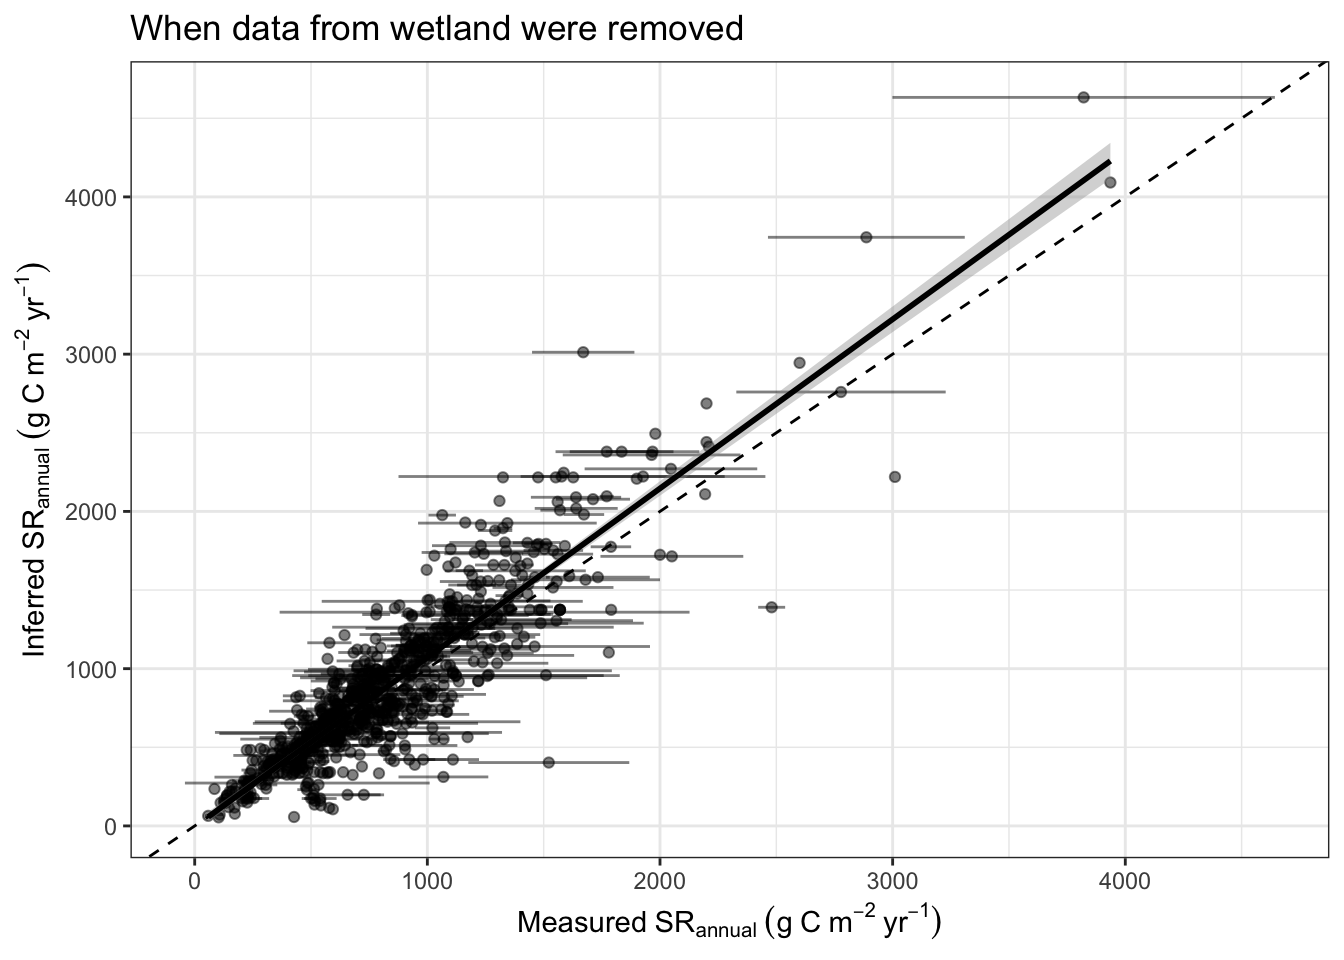
\includegraphics{6-Bahn_Analysis_Report_files/figure-latex/wetland-1.pdf}

\begin{verbatim}
## Saving 7 x 5 in image
\end{verbatim}

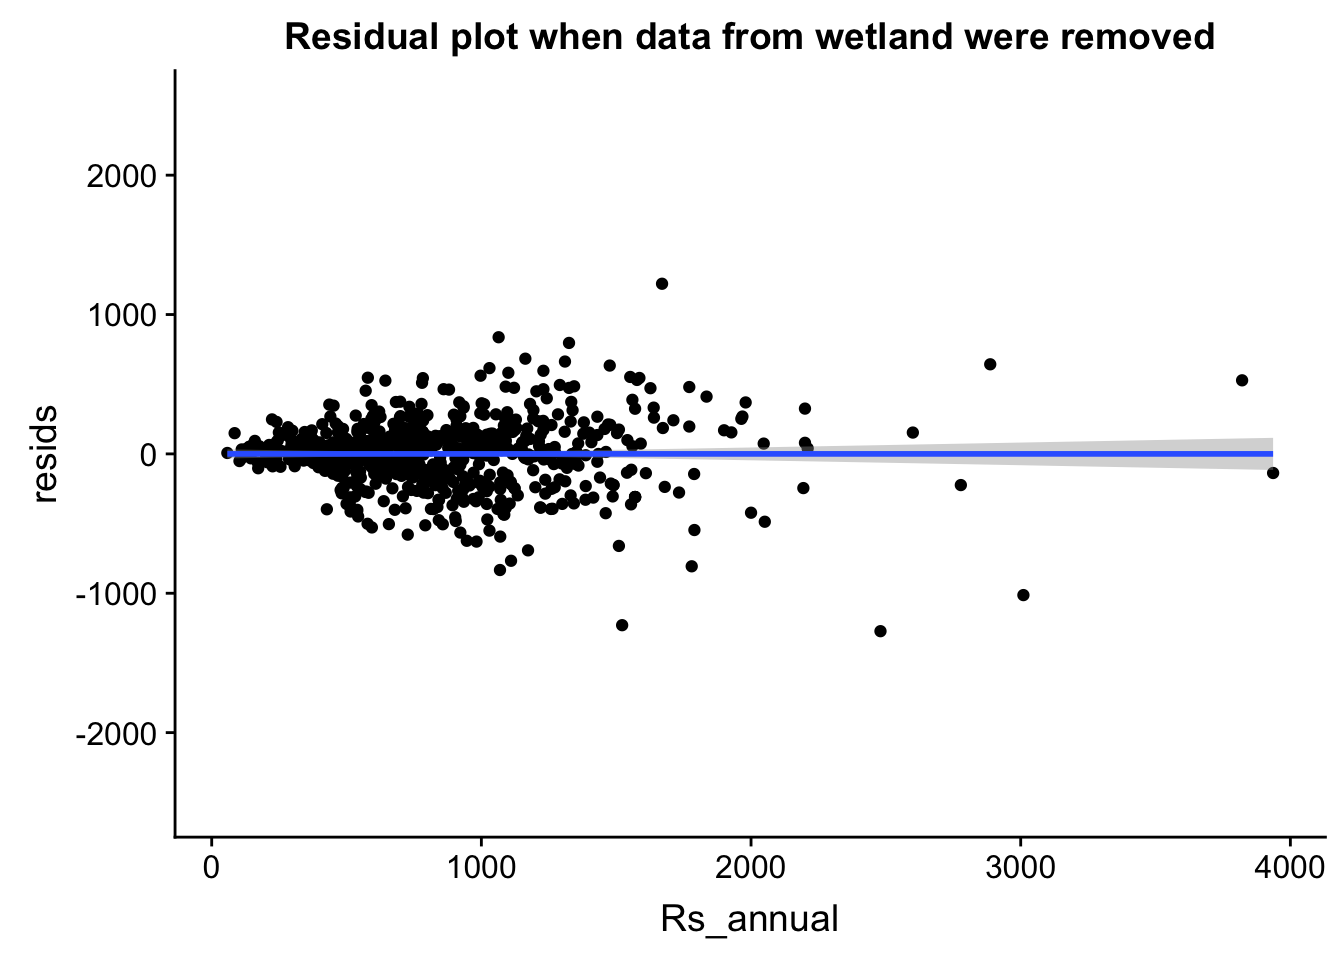
\includegraphics{6-Bahn_Analysis_Report_files/figure-latex/wetland-2.pdf}

\begin{verbatim}
## Saving 7 x 5 in image
\end{verbatim}

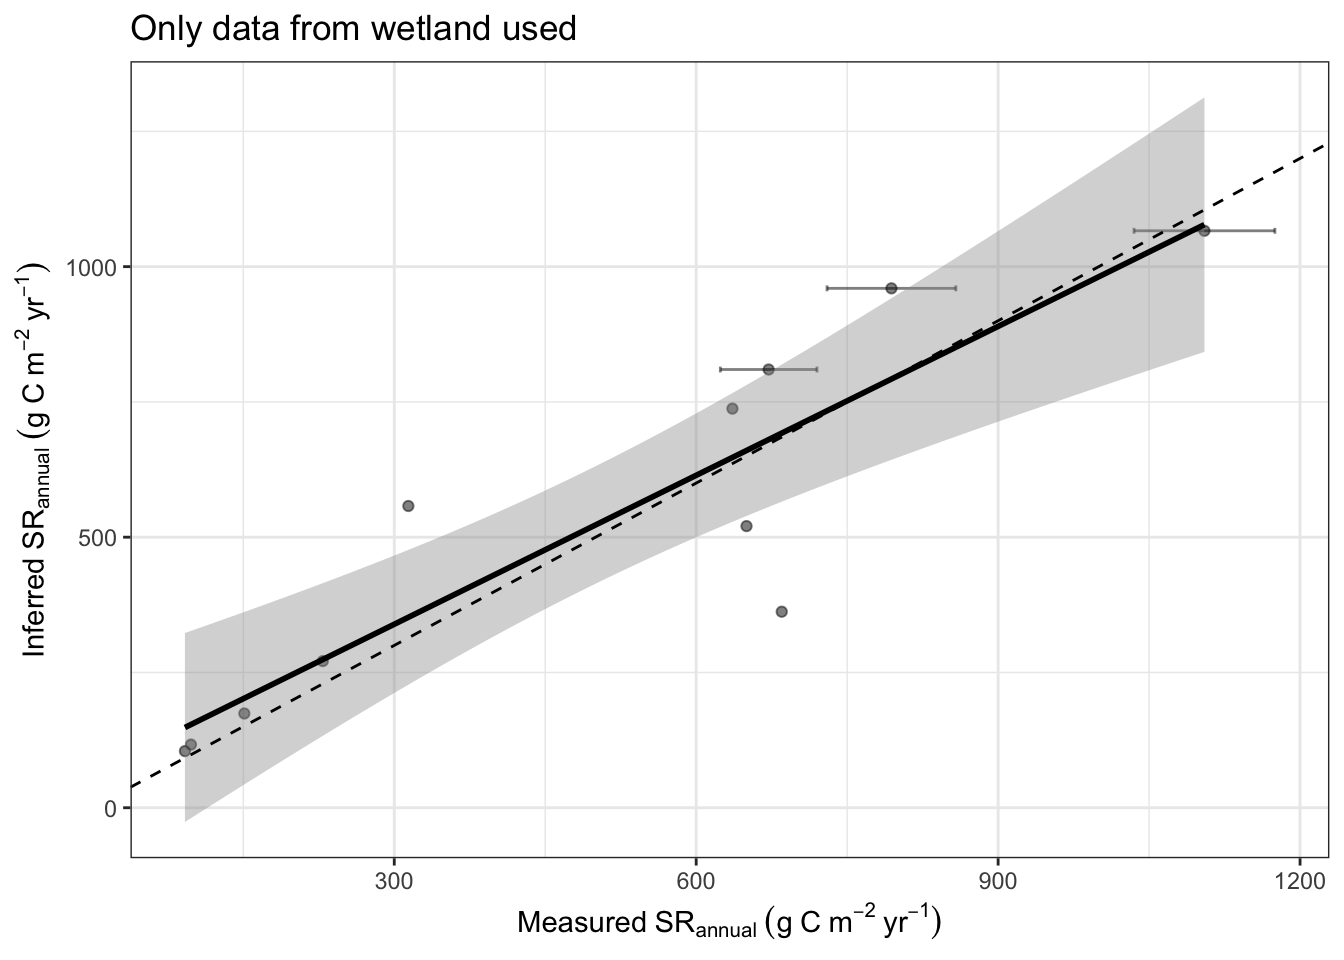
\includegraphics{6-Bahn_Analysis_Report_files/figure-latex/wetland-3.pdf}

\begin{verbatim}
## Saving 7 x 5 in image
\end{verbatim}

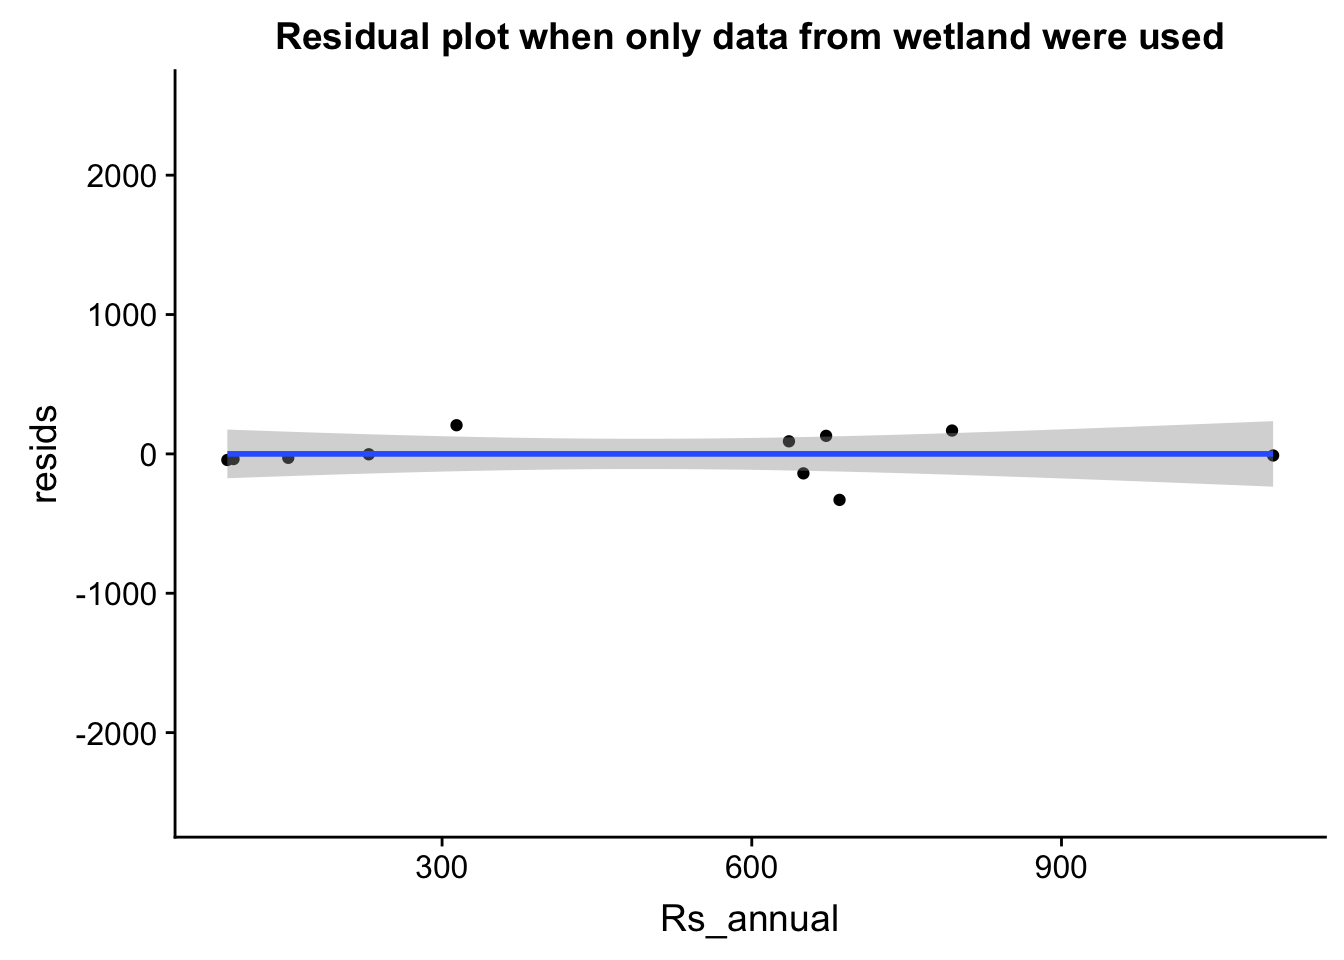
\includegraphics{6-Bahn_Analysis_Report_files/figure-latex/wetland-4.pdf}

\hypertarget{does-meas_method-affect-the-relationship}{%
\subsection{4.2.3 Does Meas\_method affect the
relationship?}\label{does-meas_method-affect-the-relationship}}

\begin{verbatim}
## Saving 7 x 5 in image
\end{verbatim}

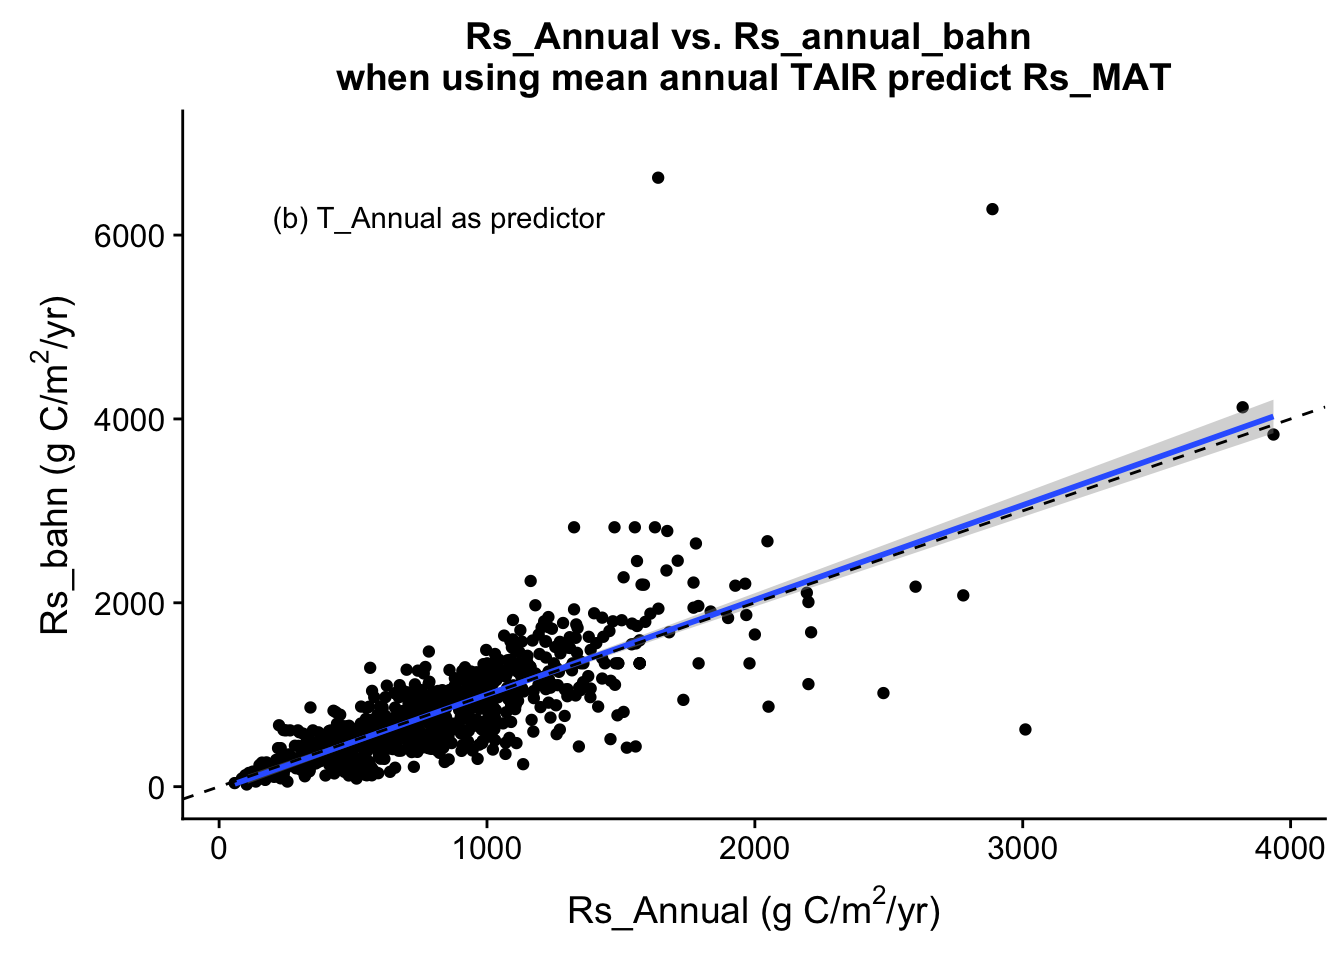
\includegraphics{6-Bahn_Analysis_Report_files/figure-latex/unnamed-chunk-13-1.pdf}

\begin{verbatim}
## Saving 7 x 5 in image
\end{verbatim}

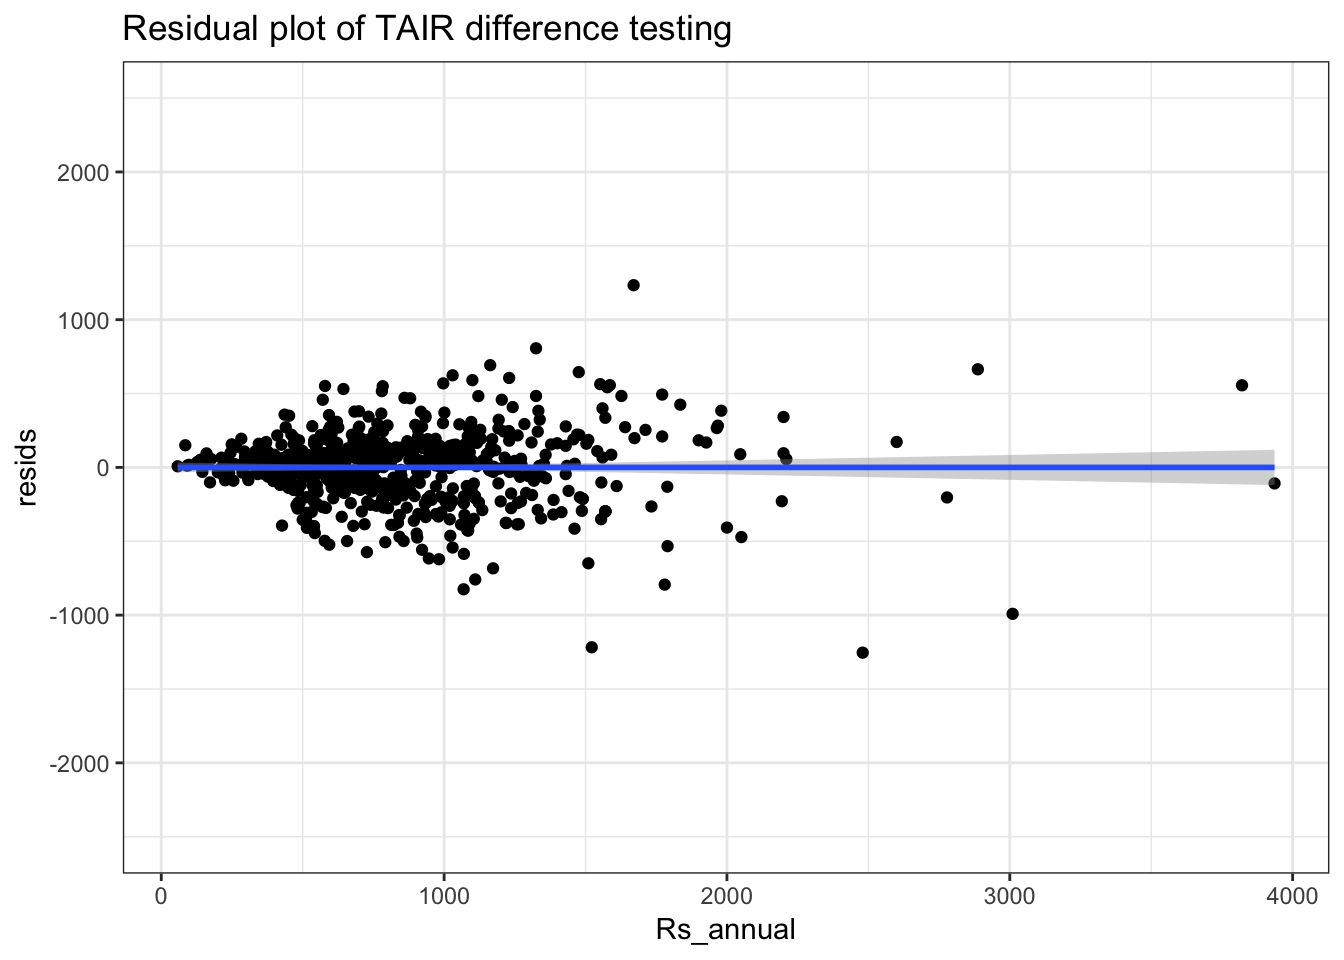
\includegraphics{6-Bahn_Analysis_Report_files/figure-latex/unnamed-chunk-13-2.pdf}

\begin{verbatim}
## Saving 7 x 5 in image
\end{verbatim}

\includegraphics{6-Bahn_Analysis_Report_files/figure-latex/unnamed-chunk-13-3.pdf}

\begin{verbatim}
## Saving 7 x 5 in image
\end{verbatim}

\includegraphics{6-Bahn_Analysis_Report_files/figure-latex/unnamed-chunk-13-4.pdf}

\hypertarget{ra--or-rh-dominated-effect}{%
\subsubsection{4.2.4 RA- or RH-dominated
effect?}\label{ra--or-rh-dominated-effect}}

\begin{verbatim}
## Saving 7 x 5 in image
\end{verbatim}

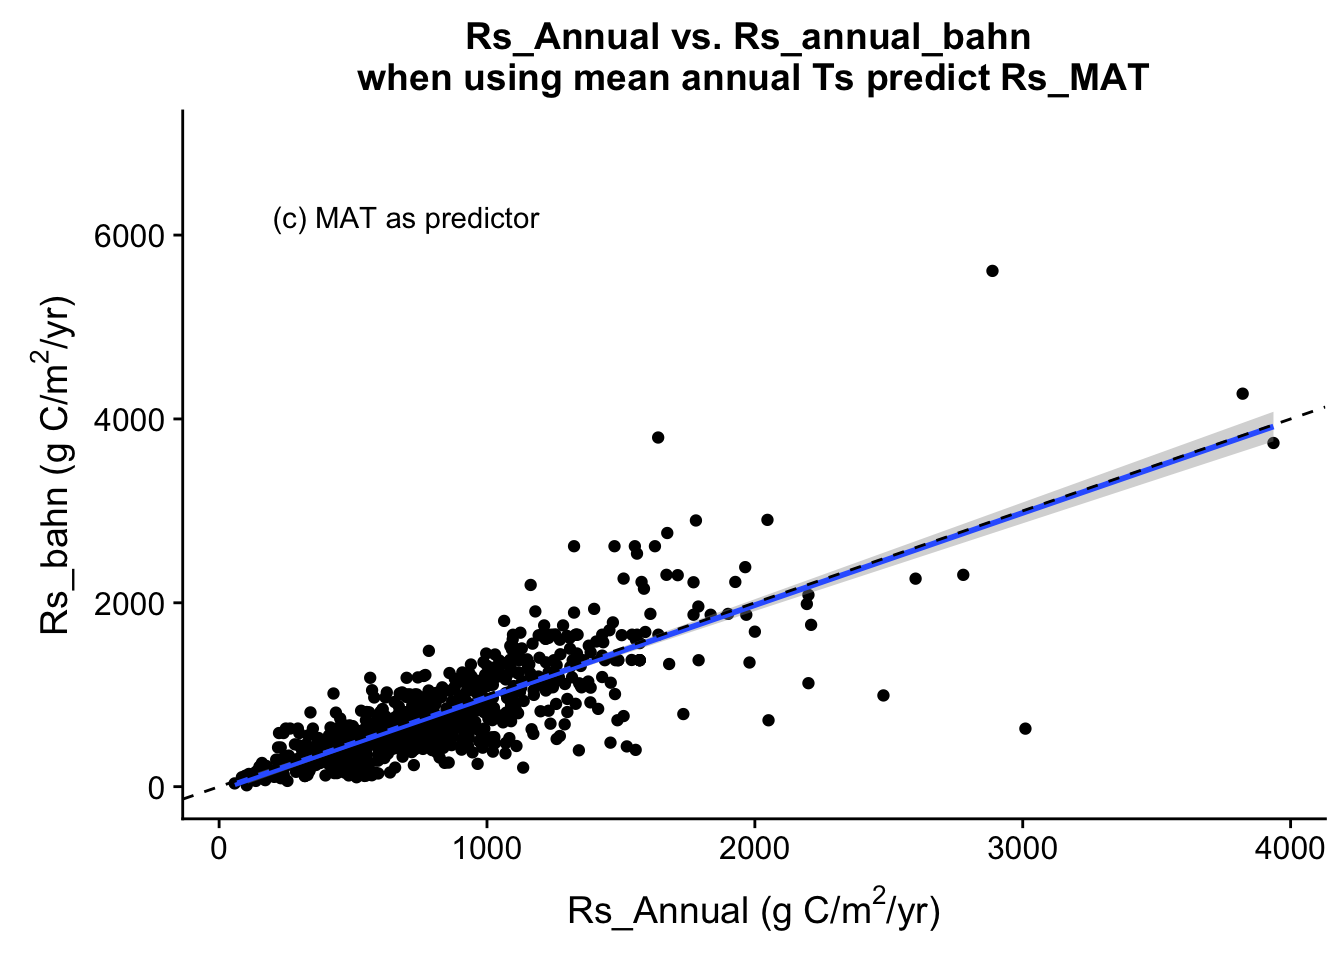
\includegraphics{6-Bahn_Analysis_Report_files/figure-latex/unnamed-chunk-14-1.pdf}

\hypertarget{biome-effect}{%
\subsubsection{4.2.5 Biome effect?}\label{biome-effect}}

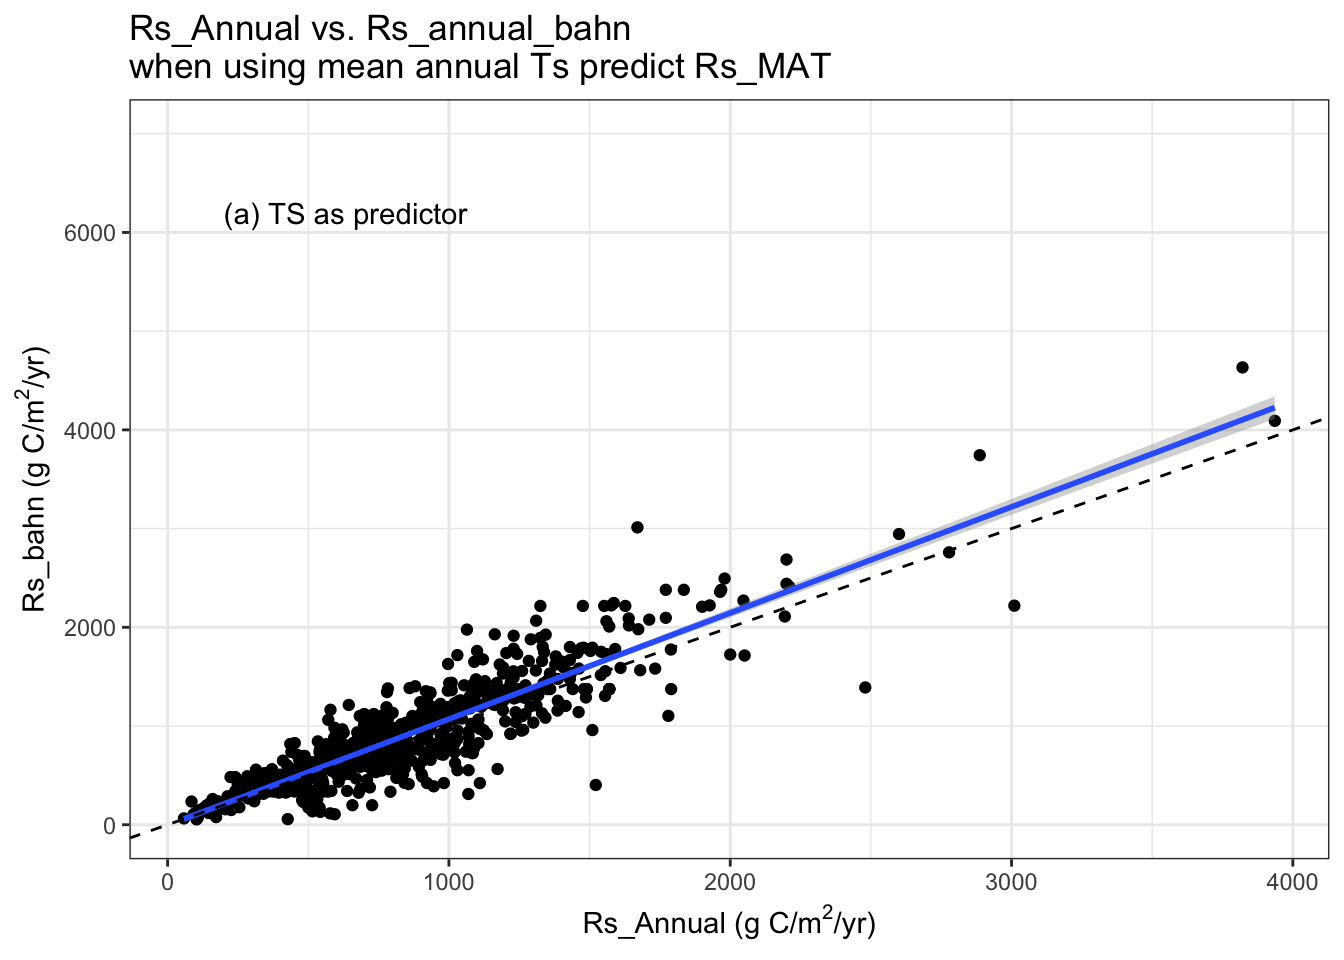
\includegraphics{6-Bahn_Analysis_Report_files/figure-latex/unnamed-chunk-15-1.pdf}

\begin{verbatim}
## geom_path: Each group consists of only one observation. Do you need to
## adjust the group aesthetic?
## geom_path: Each group consists of only one observation. Do you need to
## adjust the group aesthetic?
## geom_path: Each group consists of only one observation. Do you need to
## adjust the group aesthetic?
## geom_path: Each group consists of only one observation. Do you need to
## adjust the group aesthetic?
## geom_path: Each group consists of only one observation. Do you need to
## adjust the group aesthetic?
## geom_path: Each group consists of only one observation. Do you need to
## adjust the group aesthetic?
\end{verbatim}

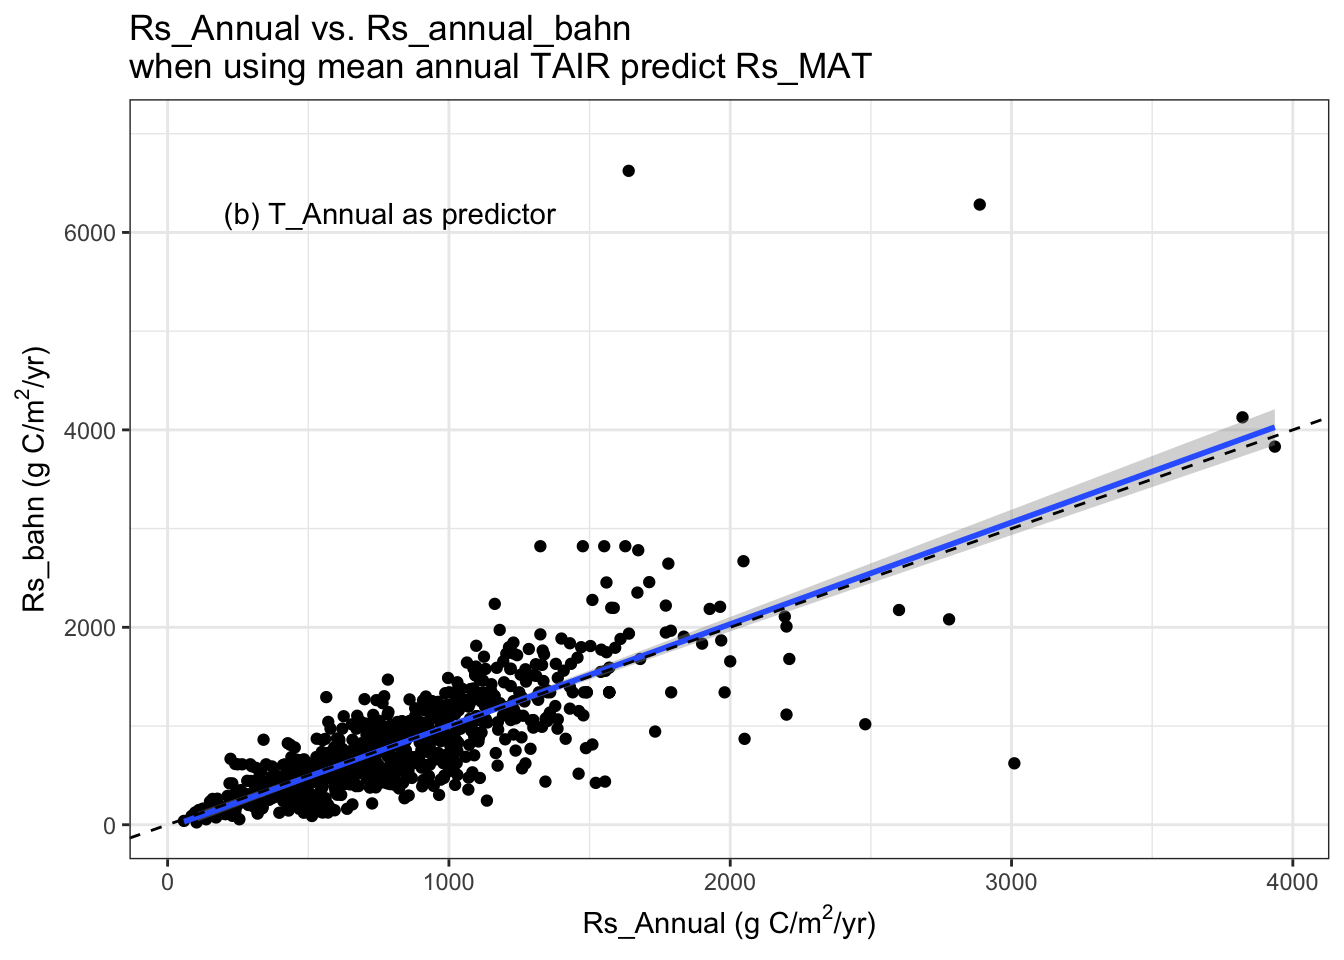
\includegraphics{6-Bahn_Analysis_Report_files/figure-latex/unnamed-chunk-16-1.pdf}

\begin{verbatim}
## geom_path: Each group consists of only one observation. Do you need to
## adjust the group aesthetic?
## geom_path: Each group consists of only one observation. Do you need to
## adjust the group aesthetic?
## geom_path: Each group consists of only one observation. Do you need to
## adjust the group aesthetic?
## geom_path: Each group consists of only one observation. Do you need to
## adjust the group aesthetic?
## geom_path: Each group consists of only one observation. Do you need to
## adjust the group aesthetic?
## geom_path: Each group consists of only one observation. Do you need to
## adjust the group aesthetic?
\end{verbatim}

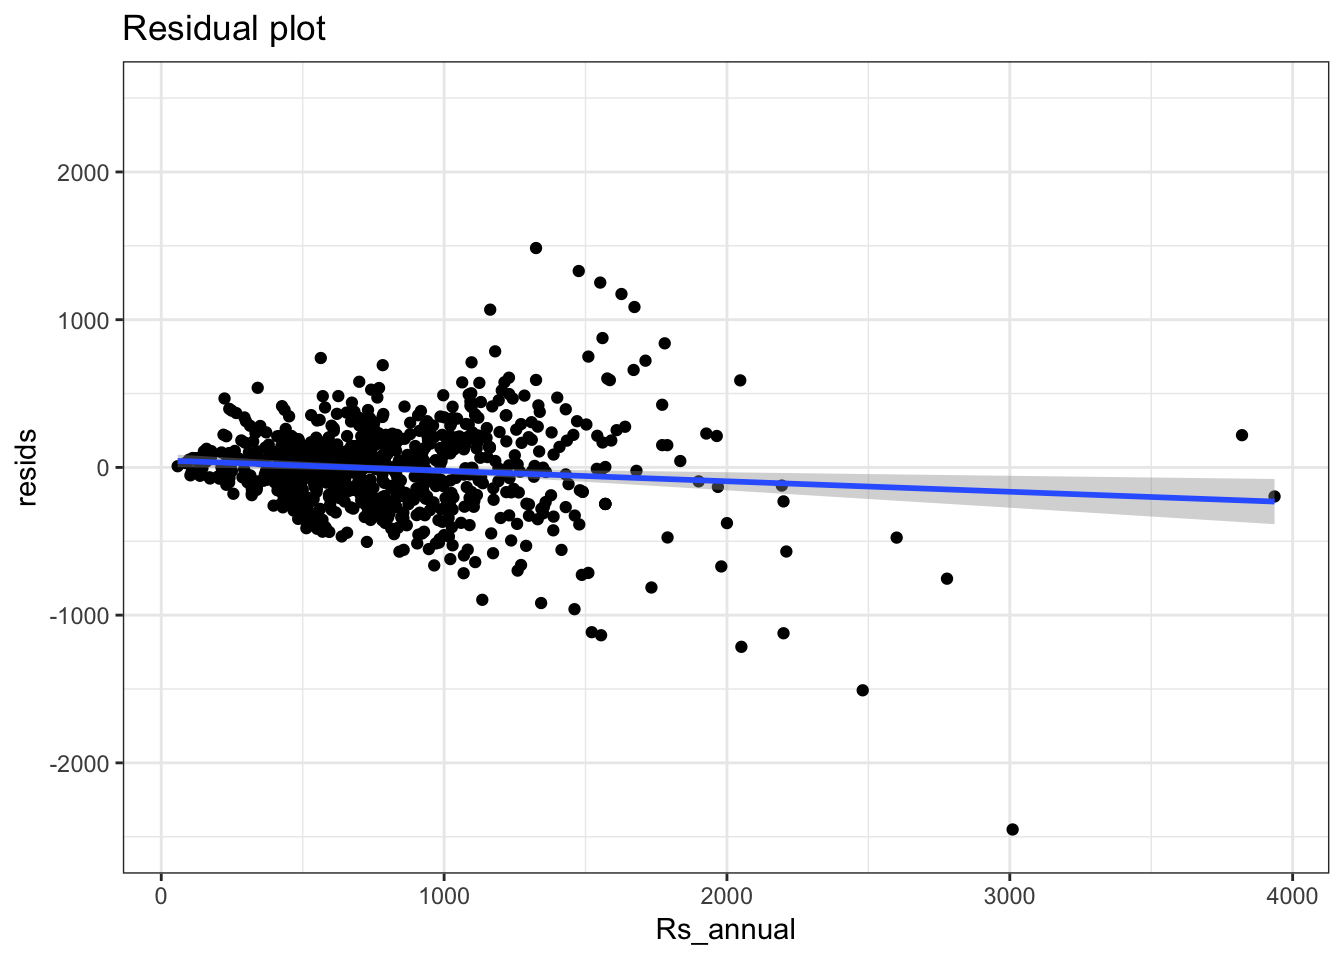
\includegraphics{6-Bahn_Analysis_Report_files/figure-latex/unnamed-chunk-16-2.pdf}

\hypertarget{tair-and-precipitation-variability-effect}{%
\subsection{4.2.6 TAIR and precipitation variability
effect?}\label{tair-and-precipitation-variability-effect}}

\begin{verbatim}
## Saving 7 x 5 in image
\end{verbatim}

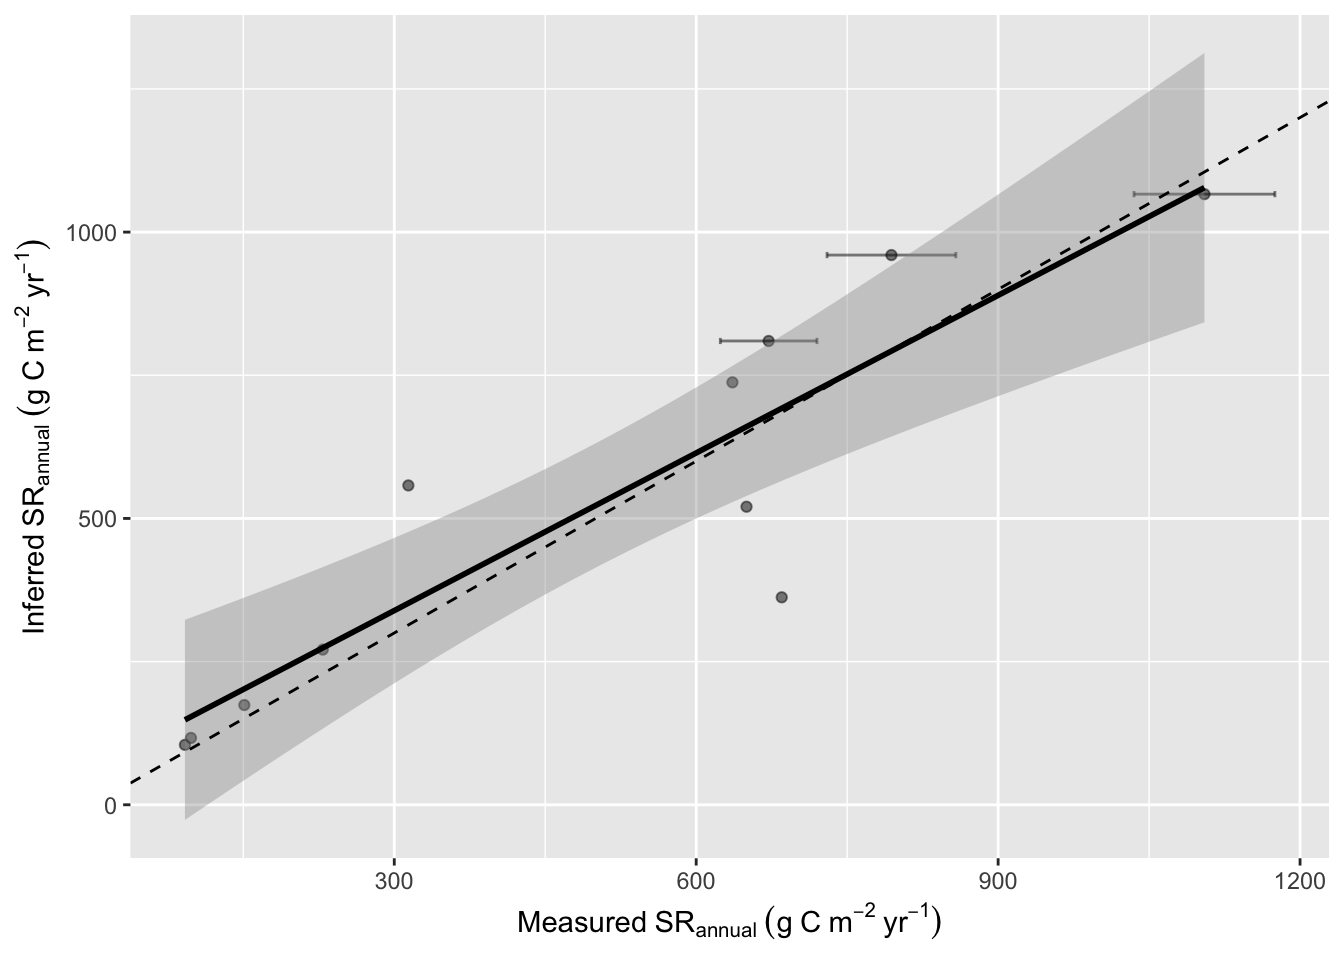
\includegraphics{6-Bahn_Analysis_Report_files/figure-latex/unnamed-chunk-17-1.pdf}

\begin{verbatim}
## Saving 7 x 5 in image
\end{verbatim}

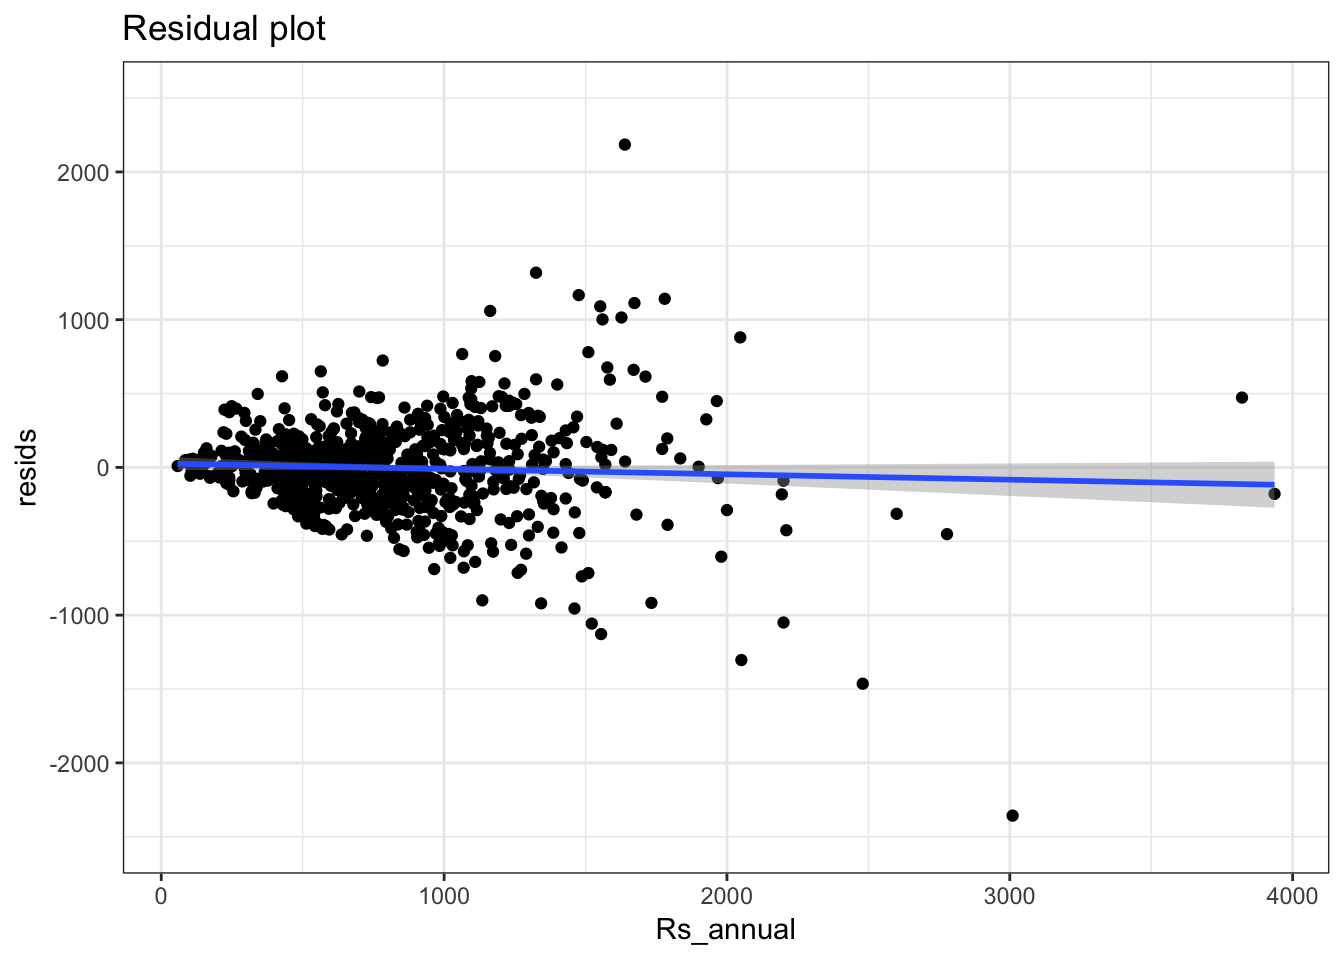
\includegraphics{6-Bahn_Analysis_Report_files/figure-latex/unnamed-chunk-17-2.pdf}

\hypertarget{drought-effect}{%
\subsection{4.2.7 Drought effect?}\label{drought-effect}}

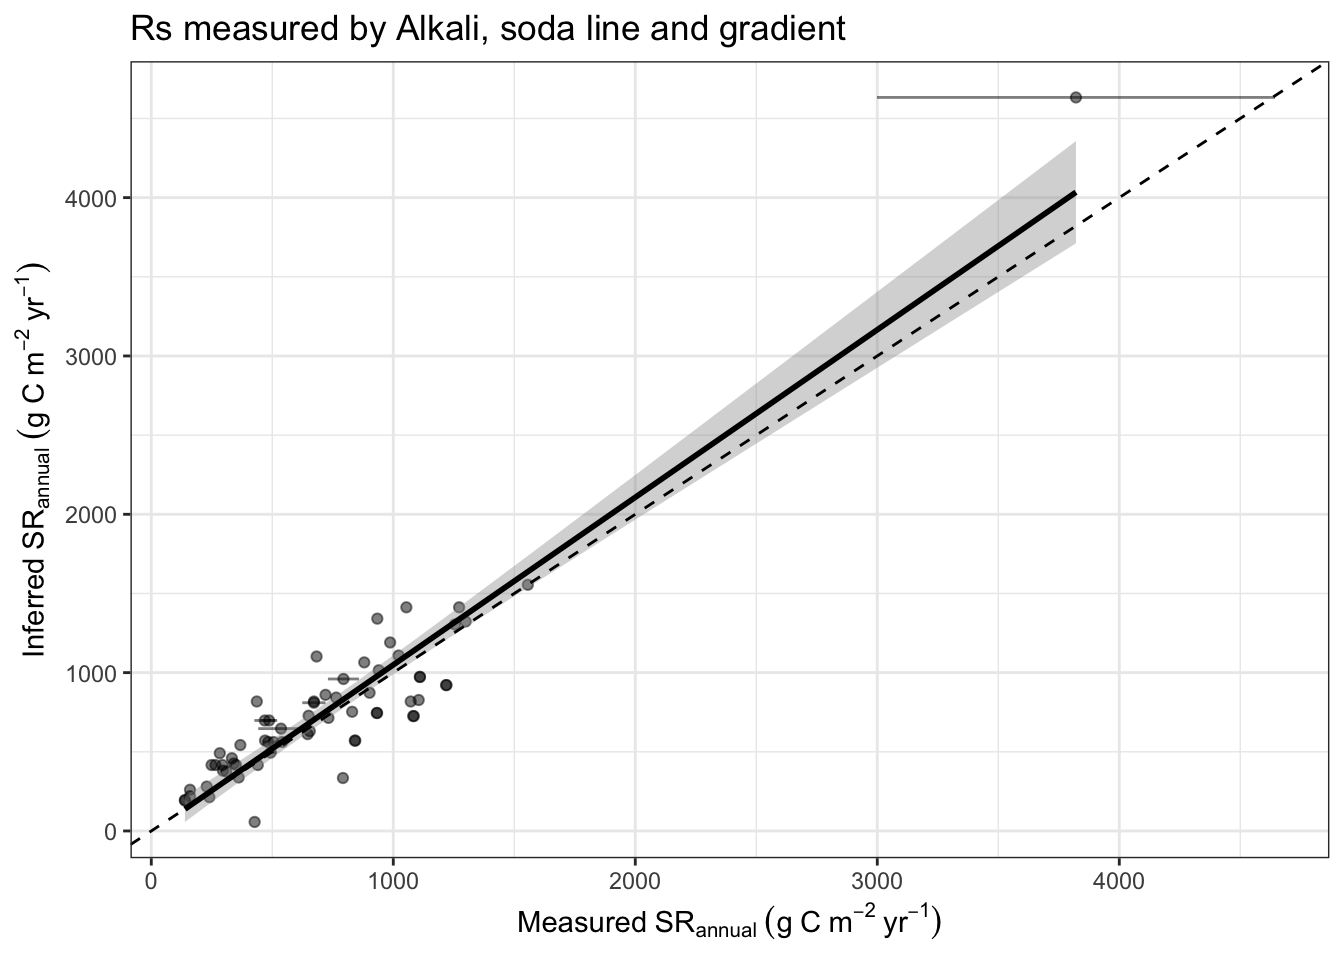
\includegraphics{6-Bahn_Analysis_Report_files/figure-latex/unnamed-chunk-18-1.pdf}

\begin{verbatim}
## Saving 7 x 5 in image
\end{verbatim}

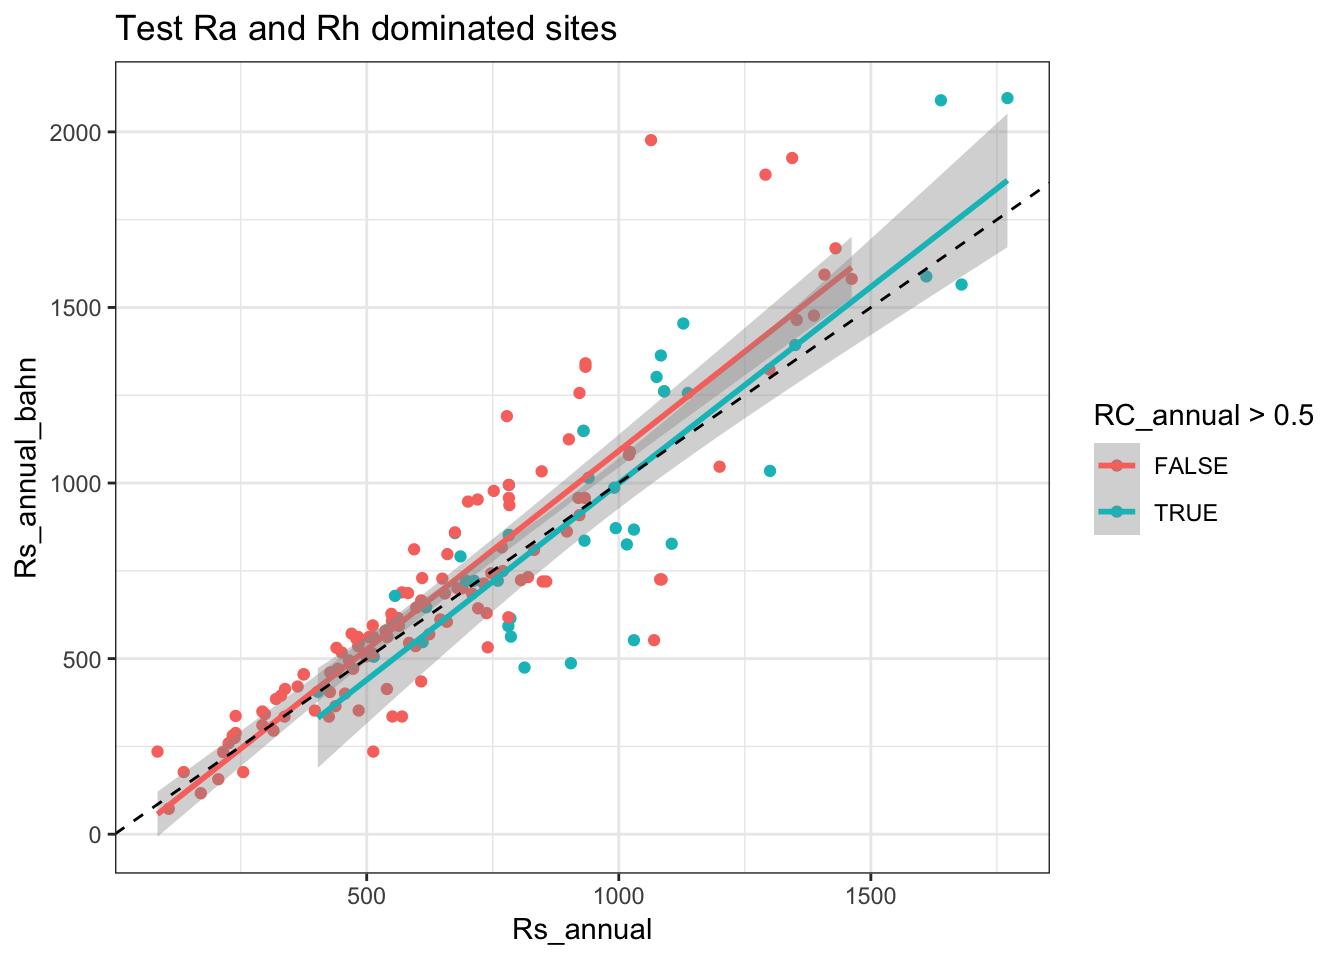
\includegraphics{6-Bahn_Analysis_Report_files/figure-latex/unnamed-chunk-19-1.pdf}

\begin{verbatim}
## Saving 7 x 5 in image
\end{verbatim}

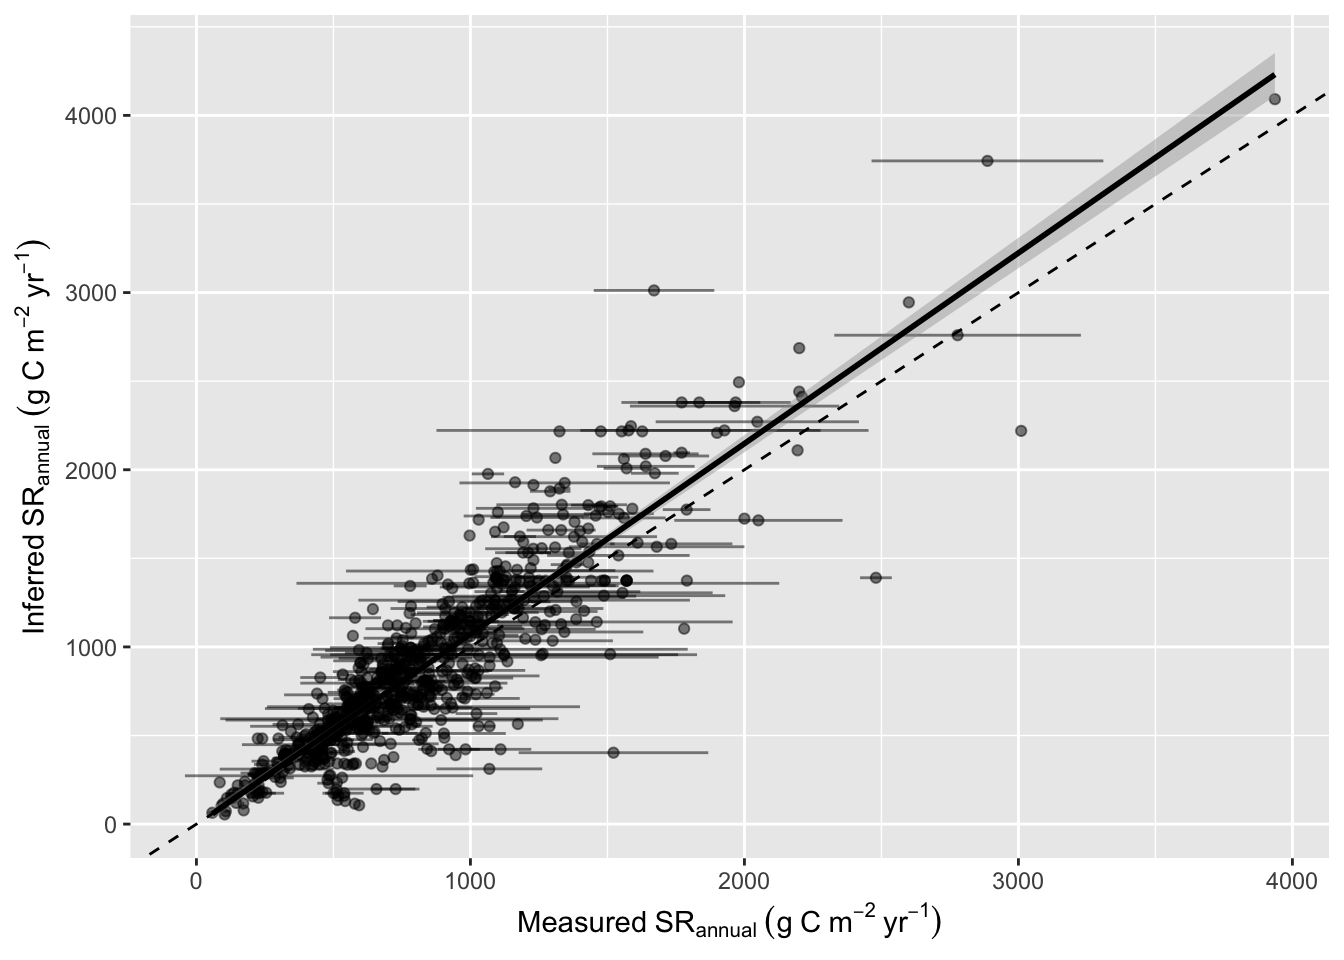
\includegraphics{6-Bahn_Analysis_Report_files/figure-latex/unnamed-chunk-20-1.pdf}

\hypertarget{discussion-questions}{%
\section{5. Discussion \& questions}\label{discussion-questions}}

\hypertarget{more-analysis-in-the-future}{%
\section{6. More analysis in the
future}\label{more-analysis-in-the-future}}

\begin{itemize}
\tightlist
\item
  1 Using SD information with boosting?
\item
  2 Use Rs\_mat predict Rh?
\item
  3 Use this approach estimate global Rs
\item
  4 Think about application
\item
  5 Update bahn model with more predictors or using regression tree
  method?
\end{itemize}


\end{document}
